\section{Analysis using additional cuts}
\label{sec:CutsAndFitterConfigs}
We examine several extra cuts in order to reduce the dominant W$jj$
background without eliminating potential new physics. In addition, we
compare the CDF-like fitter to the one configured for extracting a
diboson resonance.

\subsection{Applying anti-b-tag requirements on the two leading jets}
We tighten the anti-$b$-tag for the leading jet to a medium, high
efficiency Simple Secondary Vertex in order to eliminate the single
top background. Comparing the standard fit to the one with this cut
implemented we get a reduction, from 1179 to 592 top events. In addition,
the W$jj$ yield decreases from 29290 to 27784, while the WW yield
changes from 903 to 886 events.

\subsection{Applying cuts suggested by Eichten, Lane, and Martin (``ELM cuts'')}
We test the cuts suggested by Eichten, Lane and Martin~\cite{ELM}:
\begin{itemize}
\item $p_T(j1)>40$~GeV
\item $p_T(jj)>45$~GeV
\item $p_T(W)>60$~GeV
\item $|\Delta\eta (jj)|<1.2$
\end{itemize}
The fit results are presented in Figure~\ref{fig:ELMCutFit}. As
expected the W$jj$ yield drops from 27784 to 14178 (The WW yield goes
from 886 to 551 with the ratio of the two increasing from 0.032 to
0.039). Note that we are not applying the $Q>20$~GeV cut, as it is
specific to the $\rho_t\to W_{\pi_T}$ kinematics described in
~\cite{ELM}. Also note that requiring $p_T(W)>60$~GeV removes a large
fraction of the diboson as well as new physics signals along with
W$jj$, as shown in Figure~\ref{fig:WpTComparison} (repeating the fit
without this cut gives 729 WW and 19986 W$jj$ events).
%%%%%%%
\begin{figure}[h!] {\centering
\unitlength=0.33\linewidth
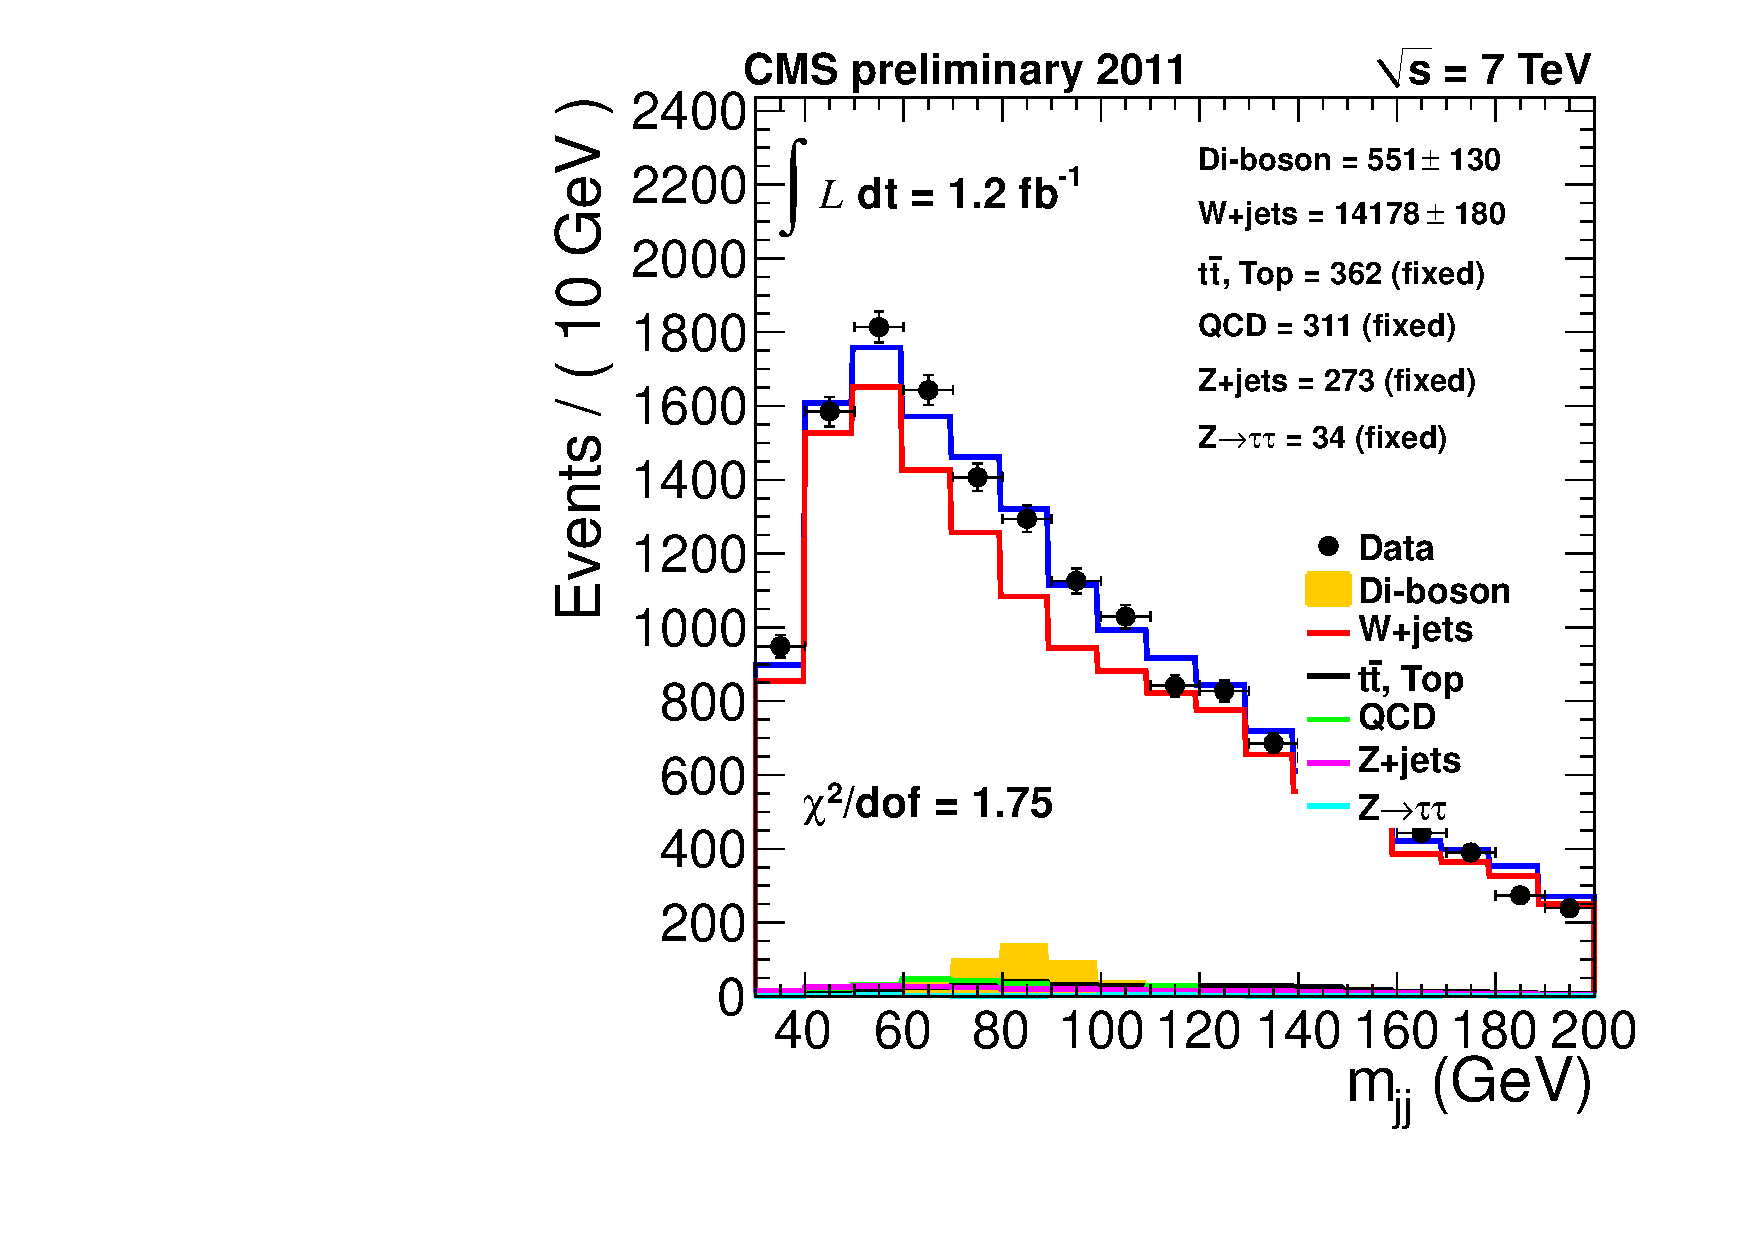
\includegraphics[width=0.48\textwidth]{figs/ELMCut_mJJ-combined-fit.pdf}
\put(-0.80,0.0){(a)} 
\unitlength=0.33\linewidth
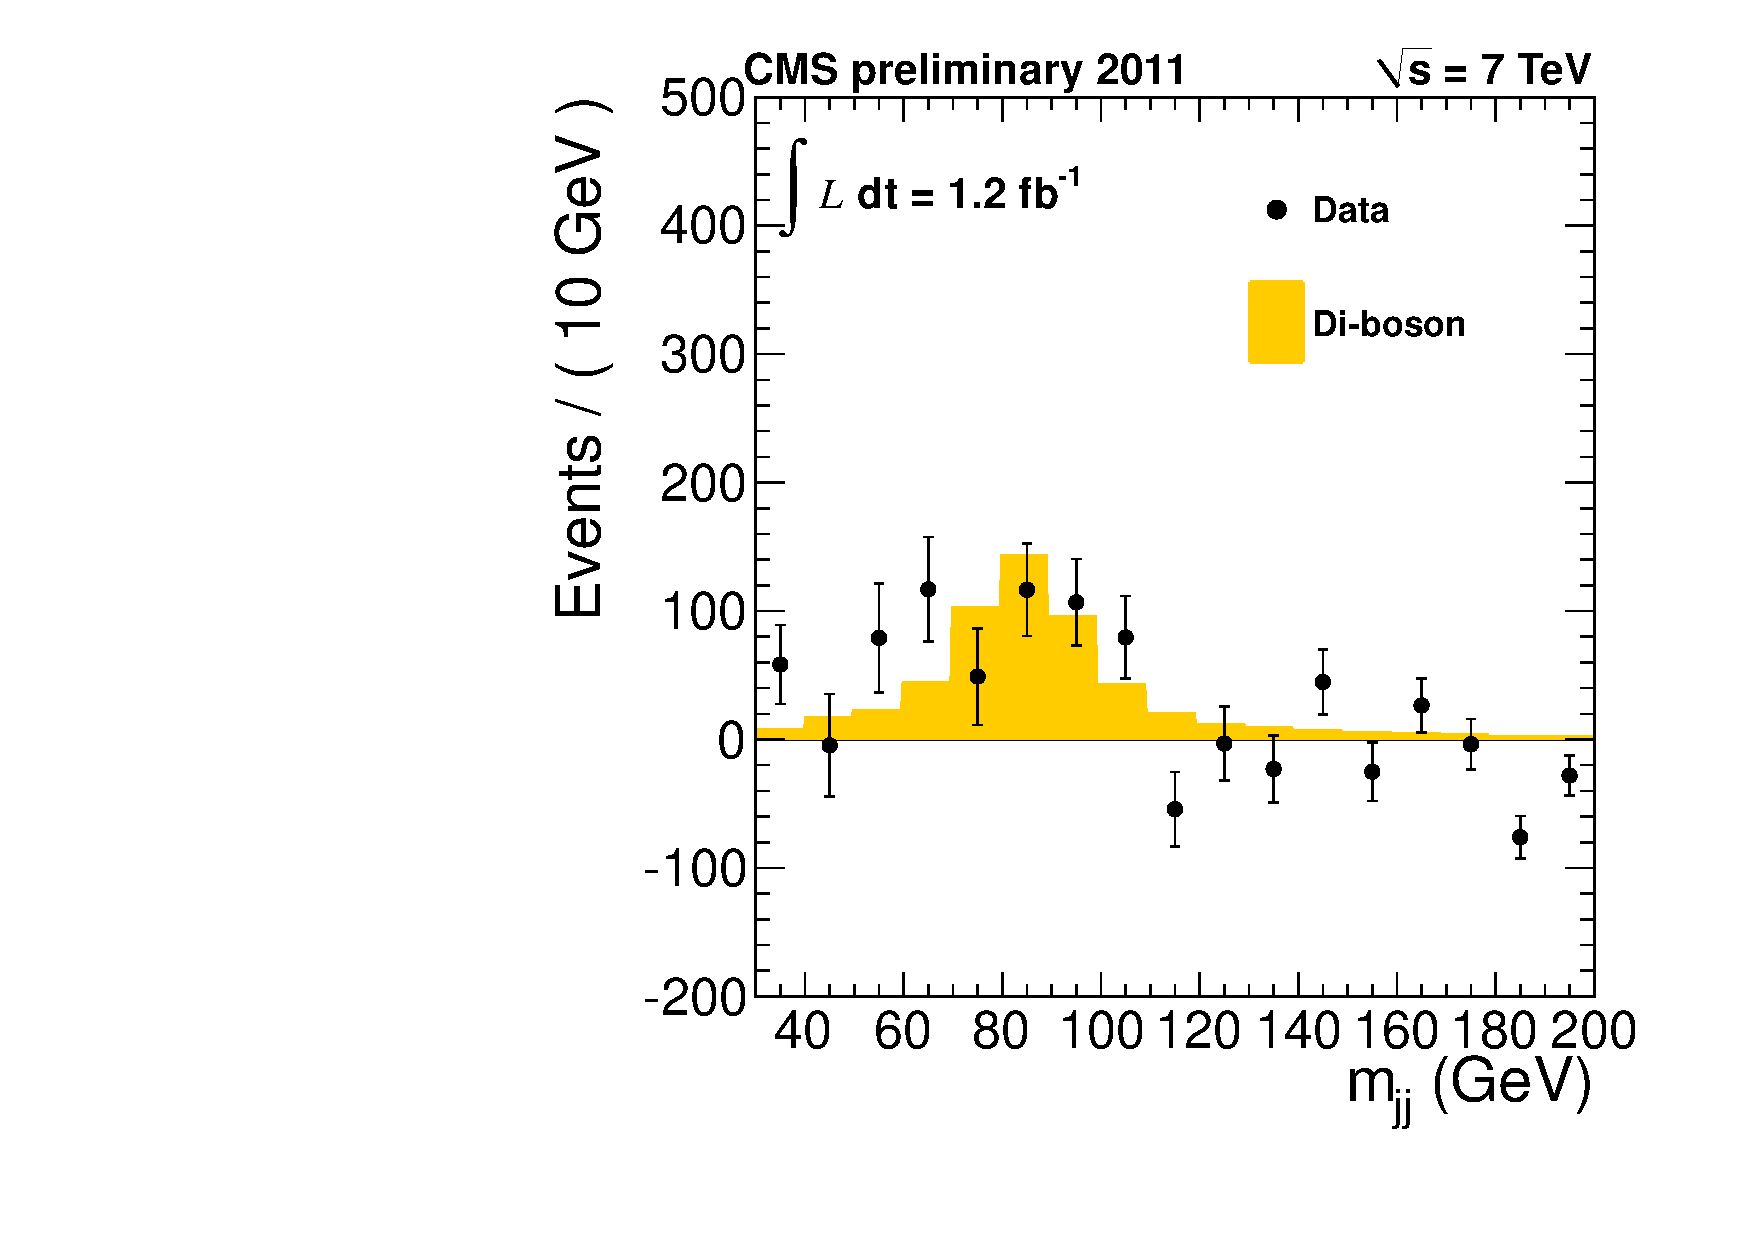
\includegraphics[width=0.48\textwidth]{figs/ELMCut_mJJ-combined-fit-subtracted.pdf}
\put(-0.80,0.0){(b)} 
\caption{Fit results with the ELM cuts $p_T(j1)>40$~GeV, $p_T(jj)>45$~GeV, $p_T(W)>60$~GeV, $|\Delta\eta (jj)|<1.2$ before (a) and after (b) the subtraction of the background components.} 
\label{fig:ELMCutFit}}
\end{figure}
%%%%%%%
\clearpage
\subsection{Investigation of the cut on Jet2pT/mjj}
\label{sec:jet2ptovermjj}
As is expected from the kinematics of the process, the sub-leading jet
${p_T}/m_{jj}$ distribution is more sharply peaked for the WW (and new
physics) resonances compared to the W$jj$ background
(Figure~\ref{fig:j2pTovermjjComparison}). Thus we place a cut of
$0.3<Jet2_{p_T}/m_{jj}<0.7$ when performing the fit, which reduces the
background. The fit results are shown in Figure~\ref{fig:J2pTomjjCutFit}.
%%%%%%%%%%%%%%%%%%%%%%%%%%%%
%%%%%%%%%%%%%%%%%%%%%%%%%%%%
%%%%%%%
\begin{figure}[h!] {\centering
\unitlength=0.33\linewidth
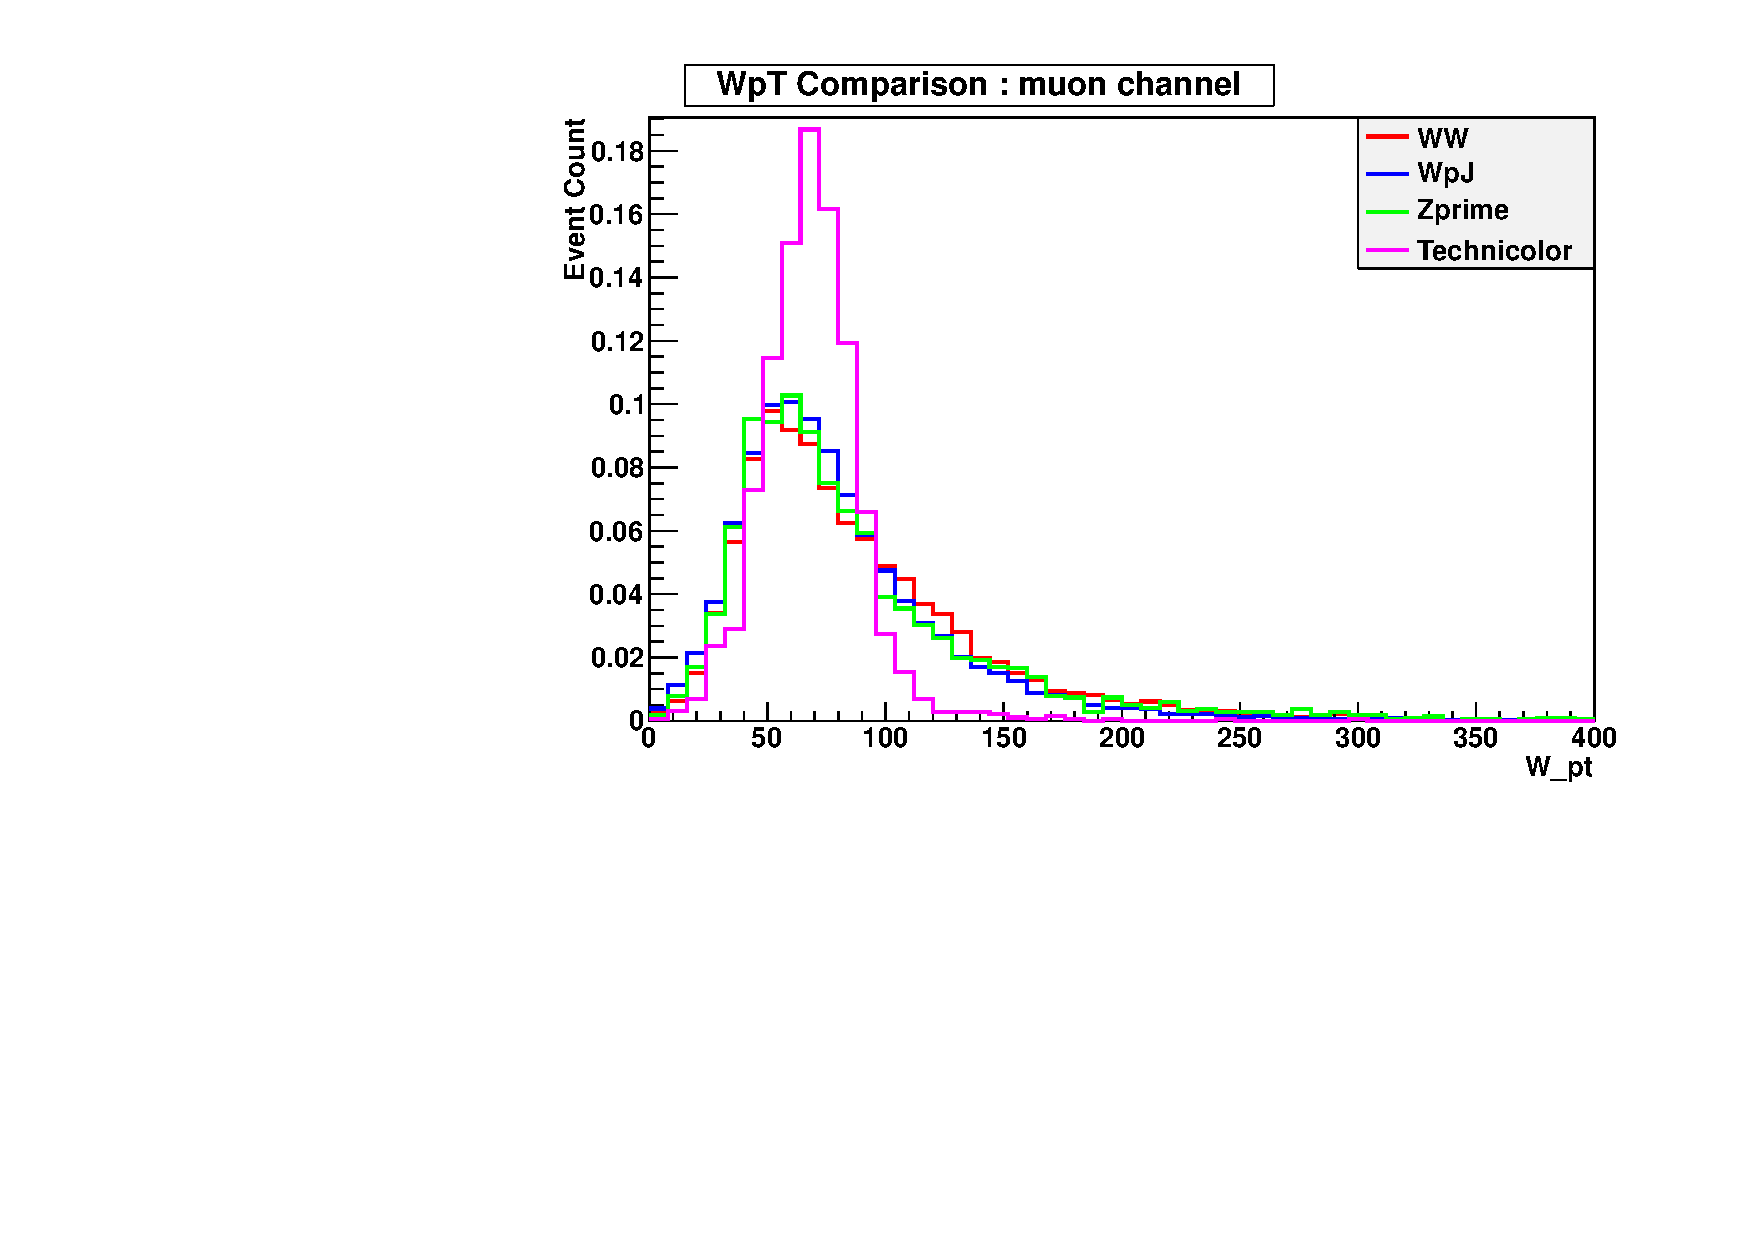
\includegraphics[width=0.48\textwidth]{figs/WpT_mu.pdf}
\put(-0.80,0.0){(a)} 
\unitlength=0.33\linewidth
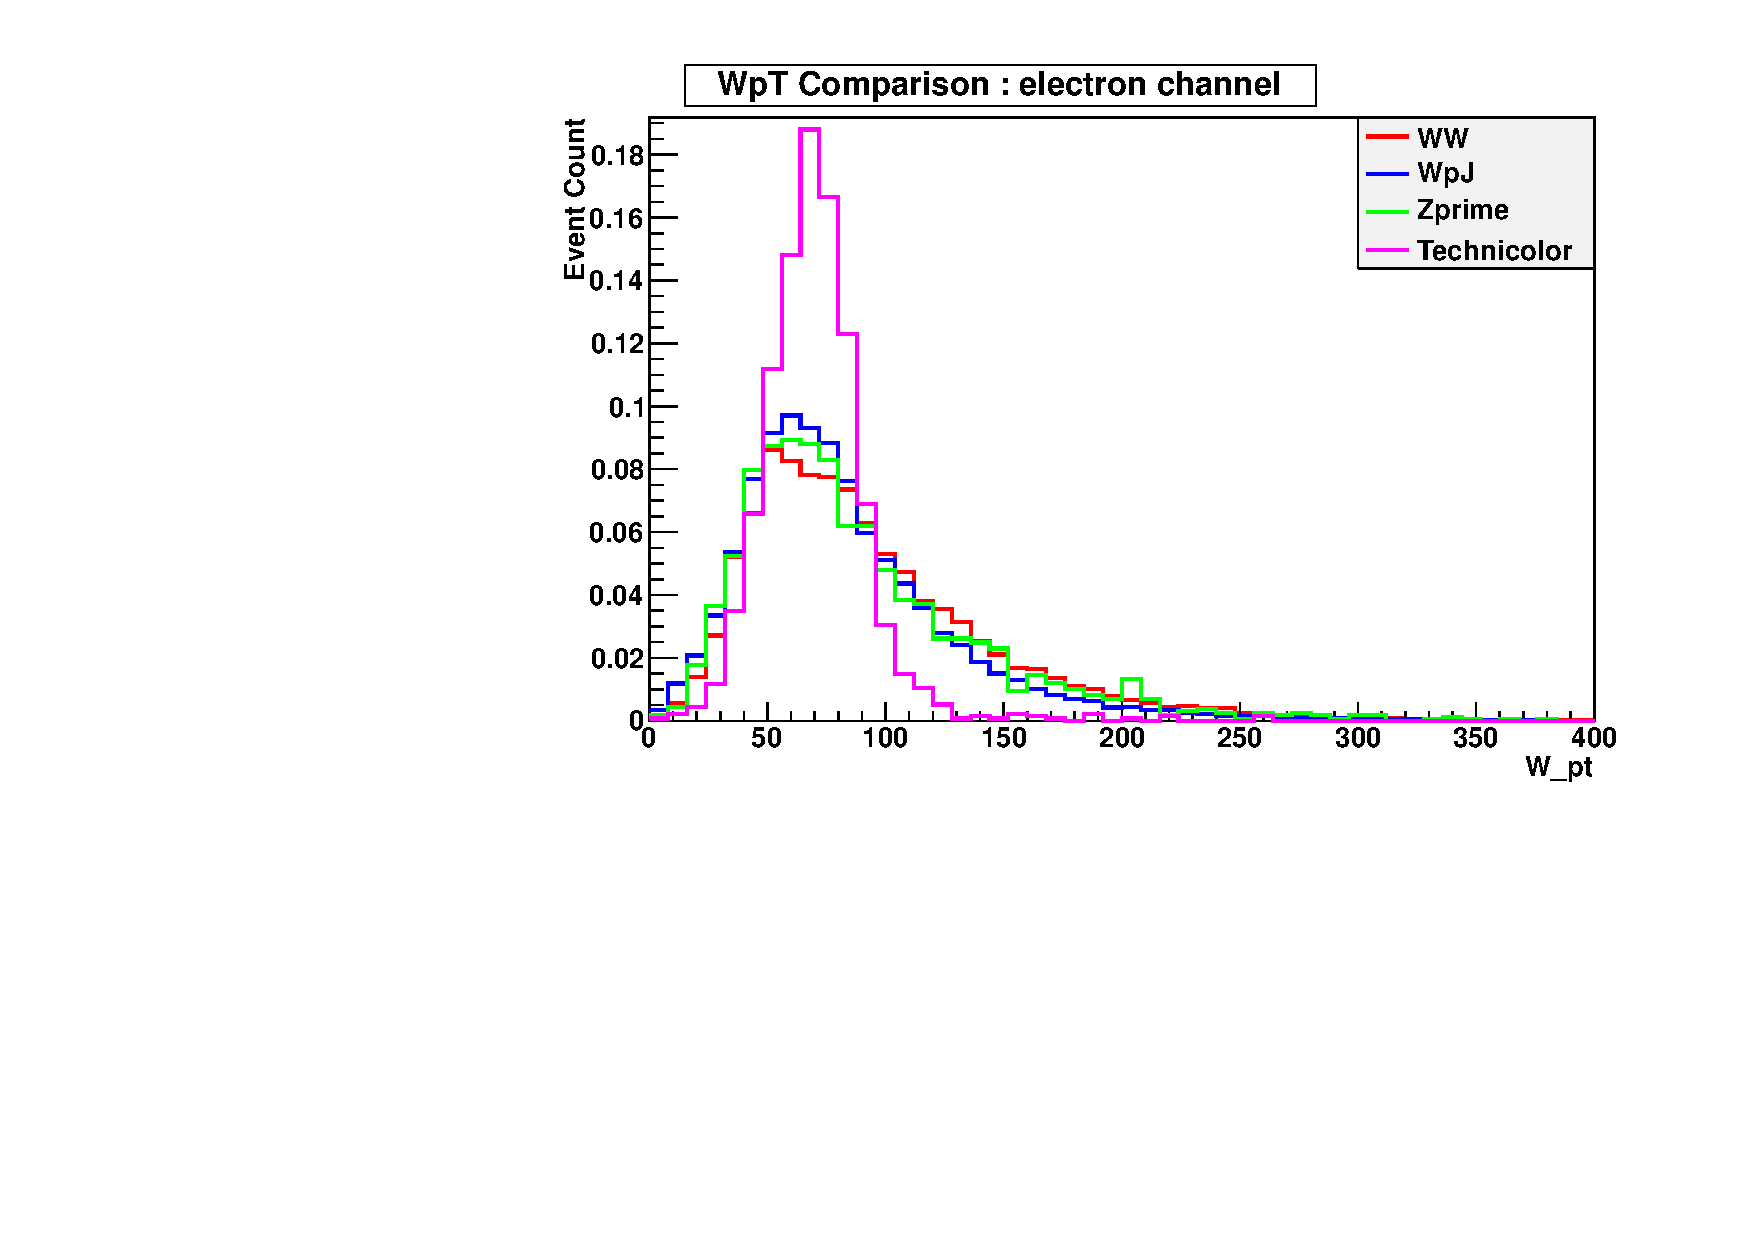
\includegraphics[width=0.48\textwidth]{figs/WpT_el.pdf}
\put(-0.80,0.0){(b)} 
\caption{$W_{p_T}$ distributions for W$jj$, WW, Z' and Technicolor Monte Carlo: (a) muons, (b) electrons.} 
\label{fig:WpTComparison}}
\end{figure}
%%%%%%%
%%%%%%%
\begin{figure}[h!] {\centering
\unitlength=0.33\linewidth
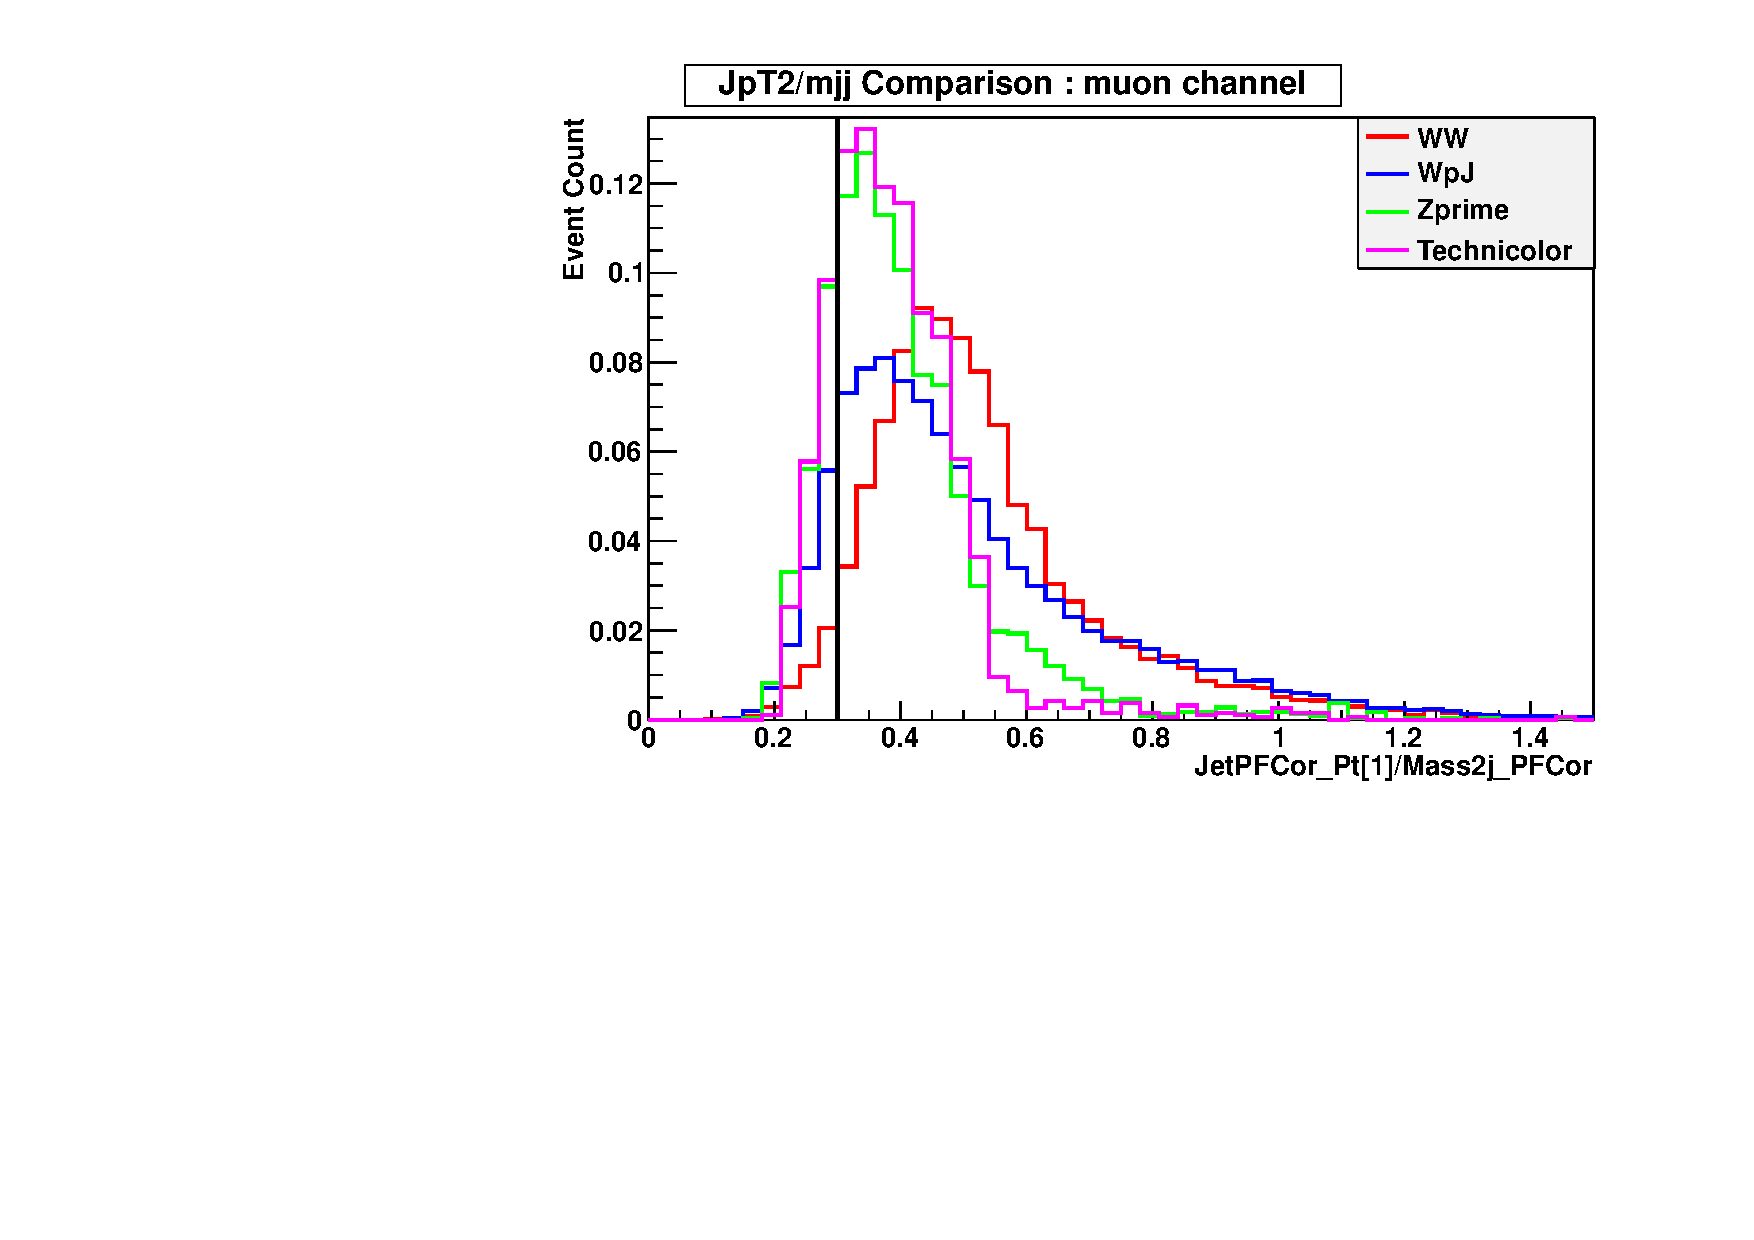
\includegraphics[width=0.48\textwidth]{figs/J2pTomjj_mu.pdf}
\put(-0.80,0.0){(a)} 
\unitlength=0.33\linewidth
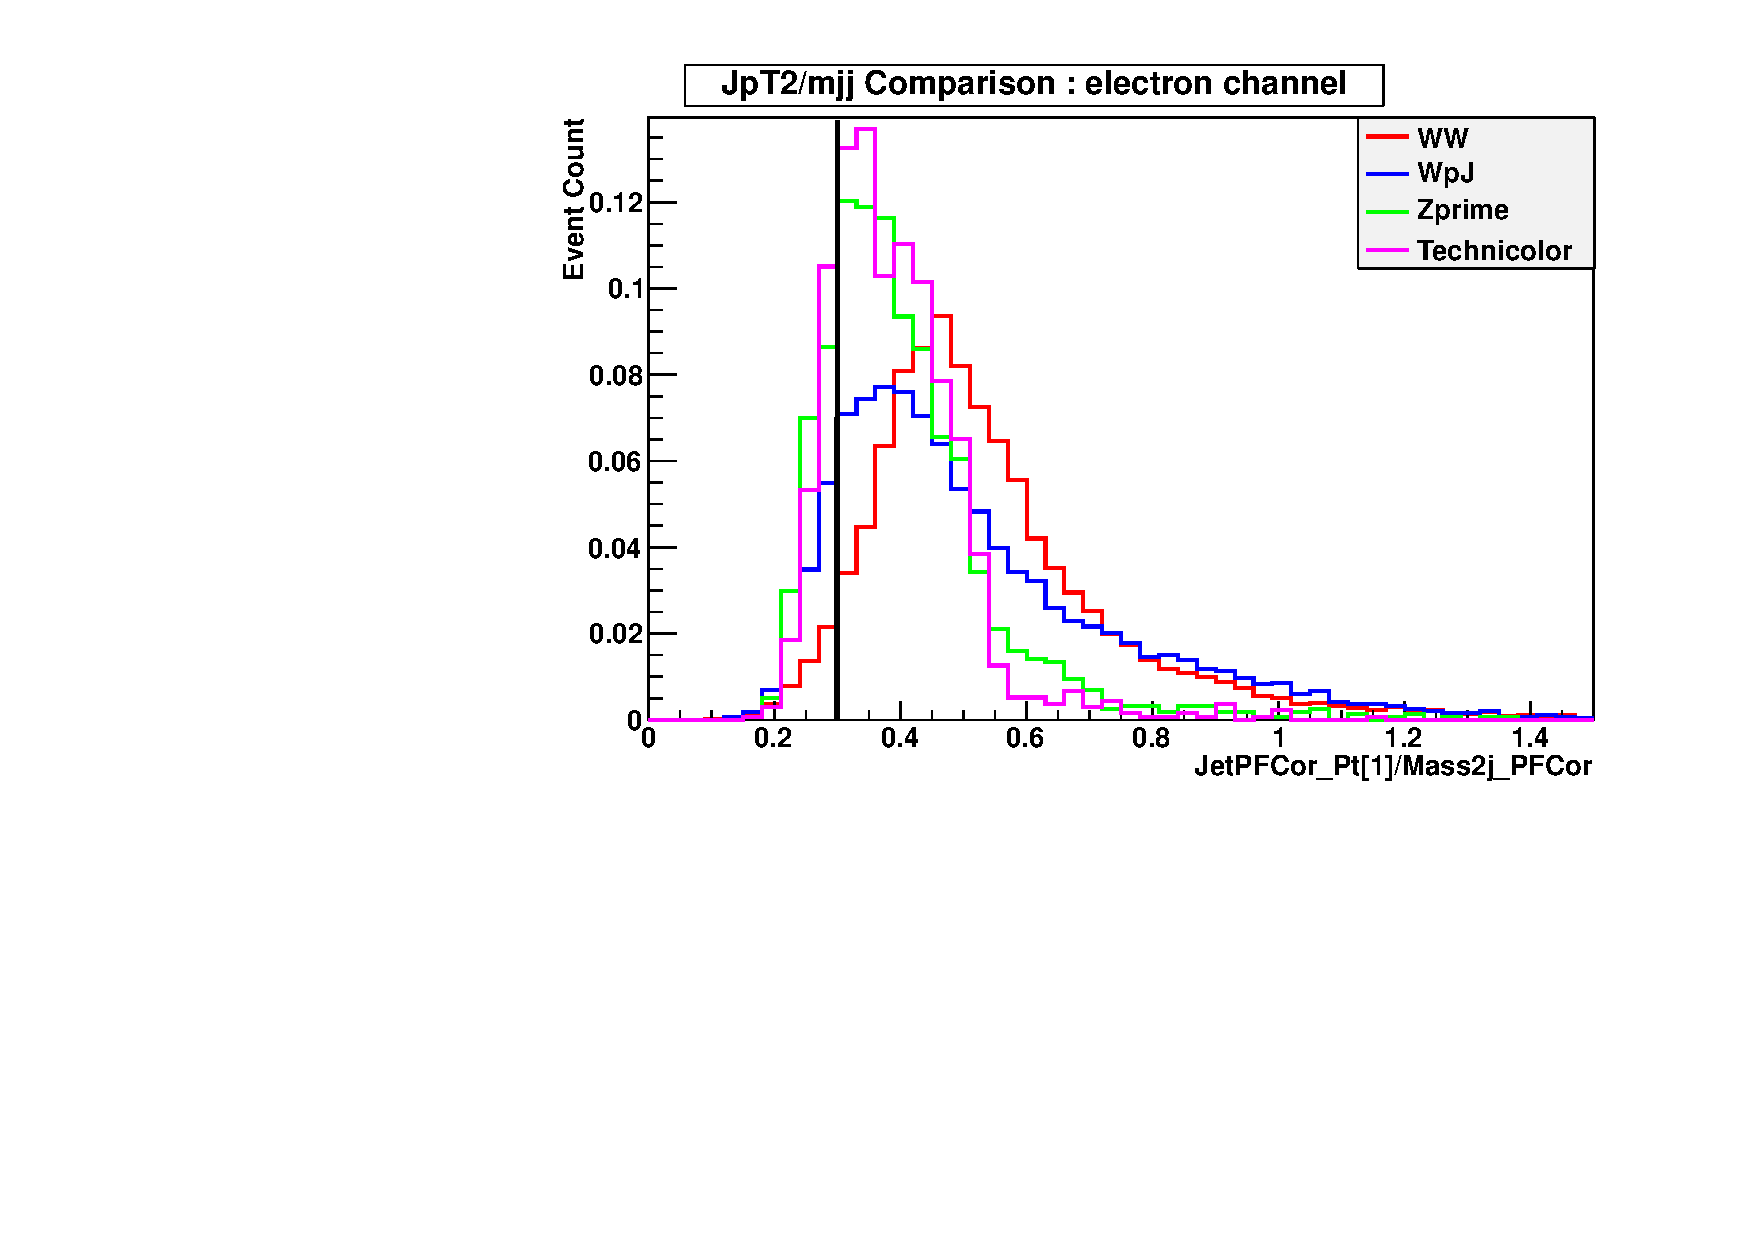
\includegraphics[width=0.48\textwidth]{figs/J2pTomjj_el.pdf}
\put(-0.80,0.0){(b)} 
\caption{$Jet2_{p_T}/m_{jj}$ distributions for W$jj$, WW, Z' and Technicolor Monte Carlo: (a) muons, (b) electrons.} 
\label{fig:j2pTovermjjComparison}}
\end{figure}
%%%%%%%
%%%%%%%
\begin{figure}[h!] {\centering
\unitlength=0.33\linewidth
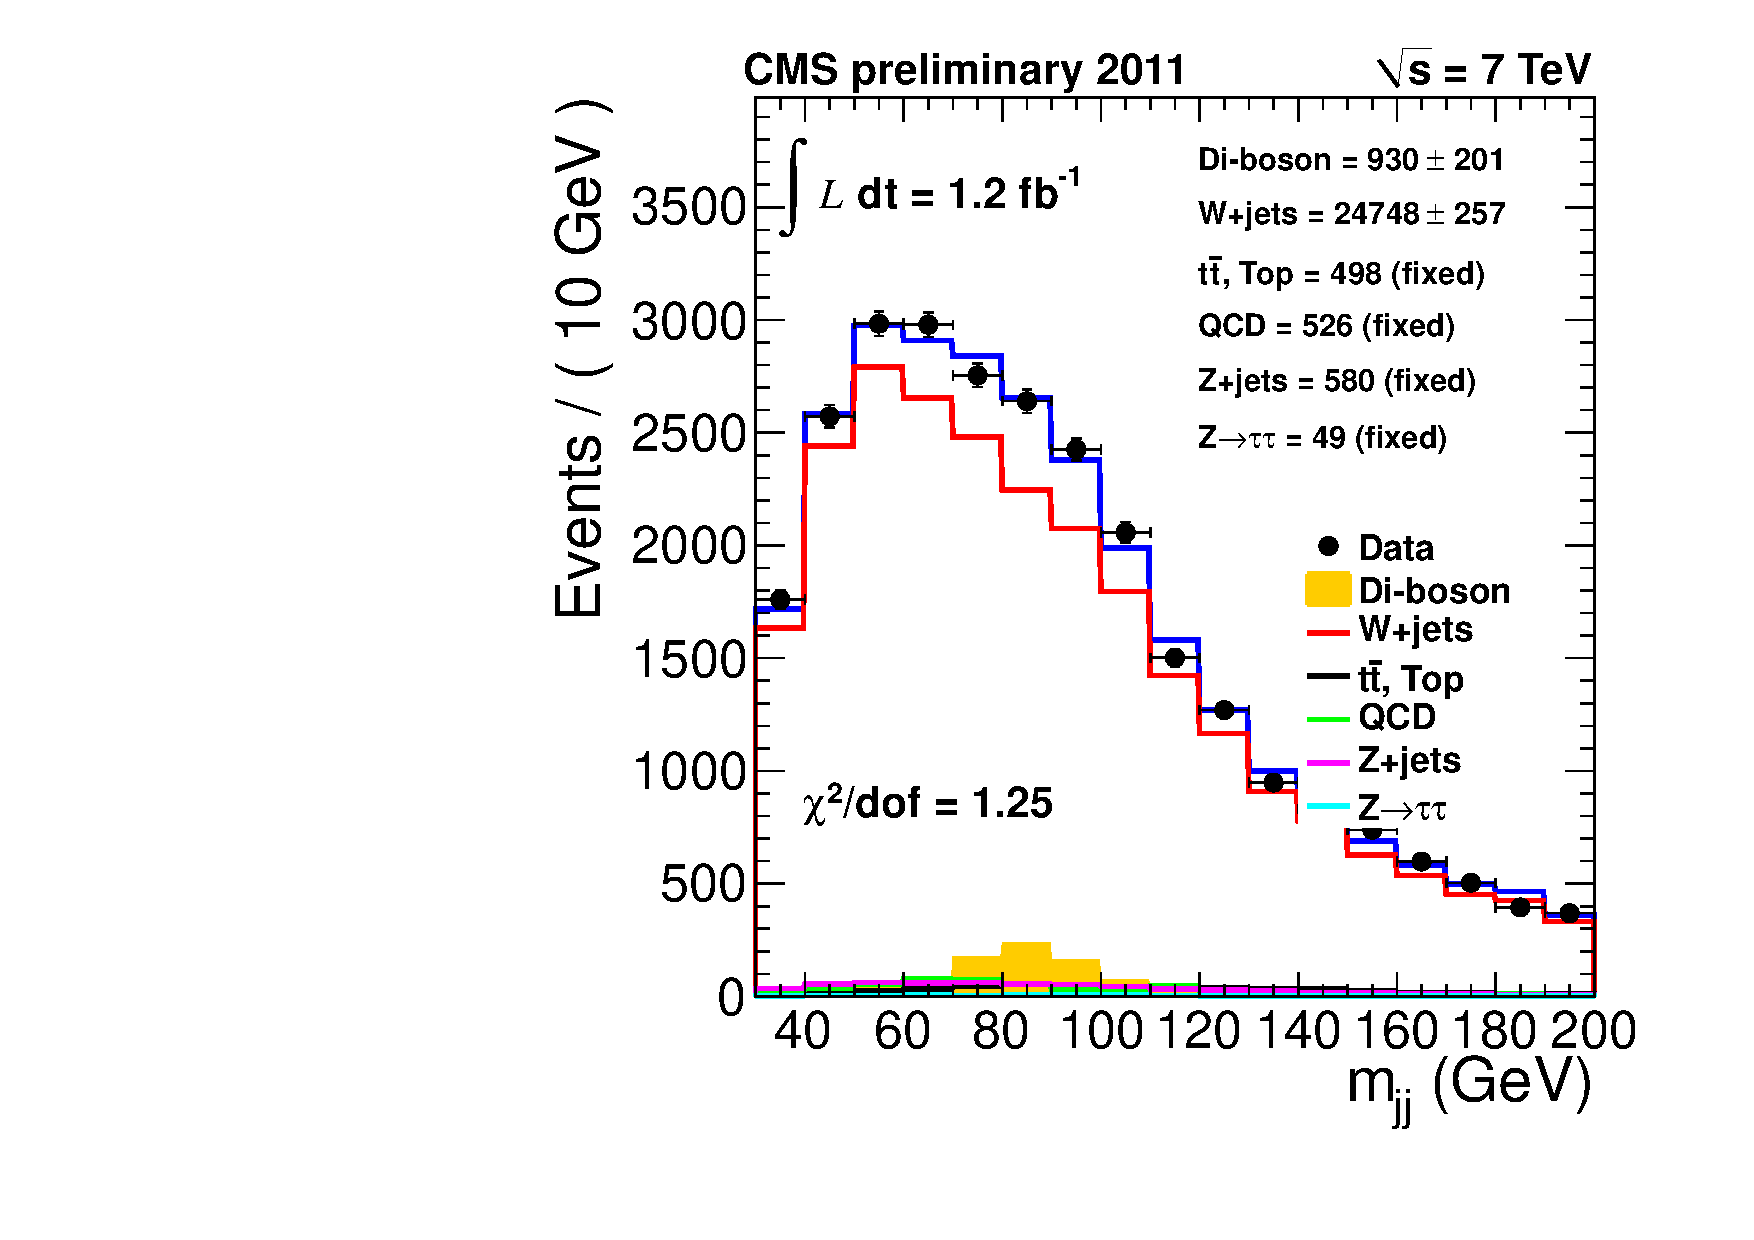
\includegraphics[width=0.48\textwidth]{figs/J2pTomjj_mJJ-combined-fit.pdf}
\put(-0.80,0.0){(a)} 
\unitlength=0.33\linewidth
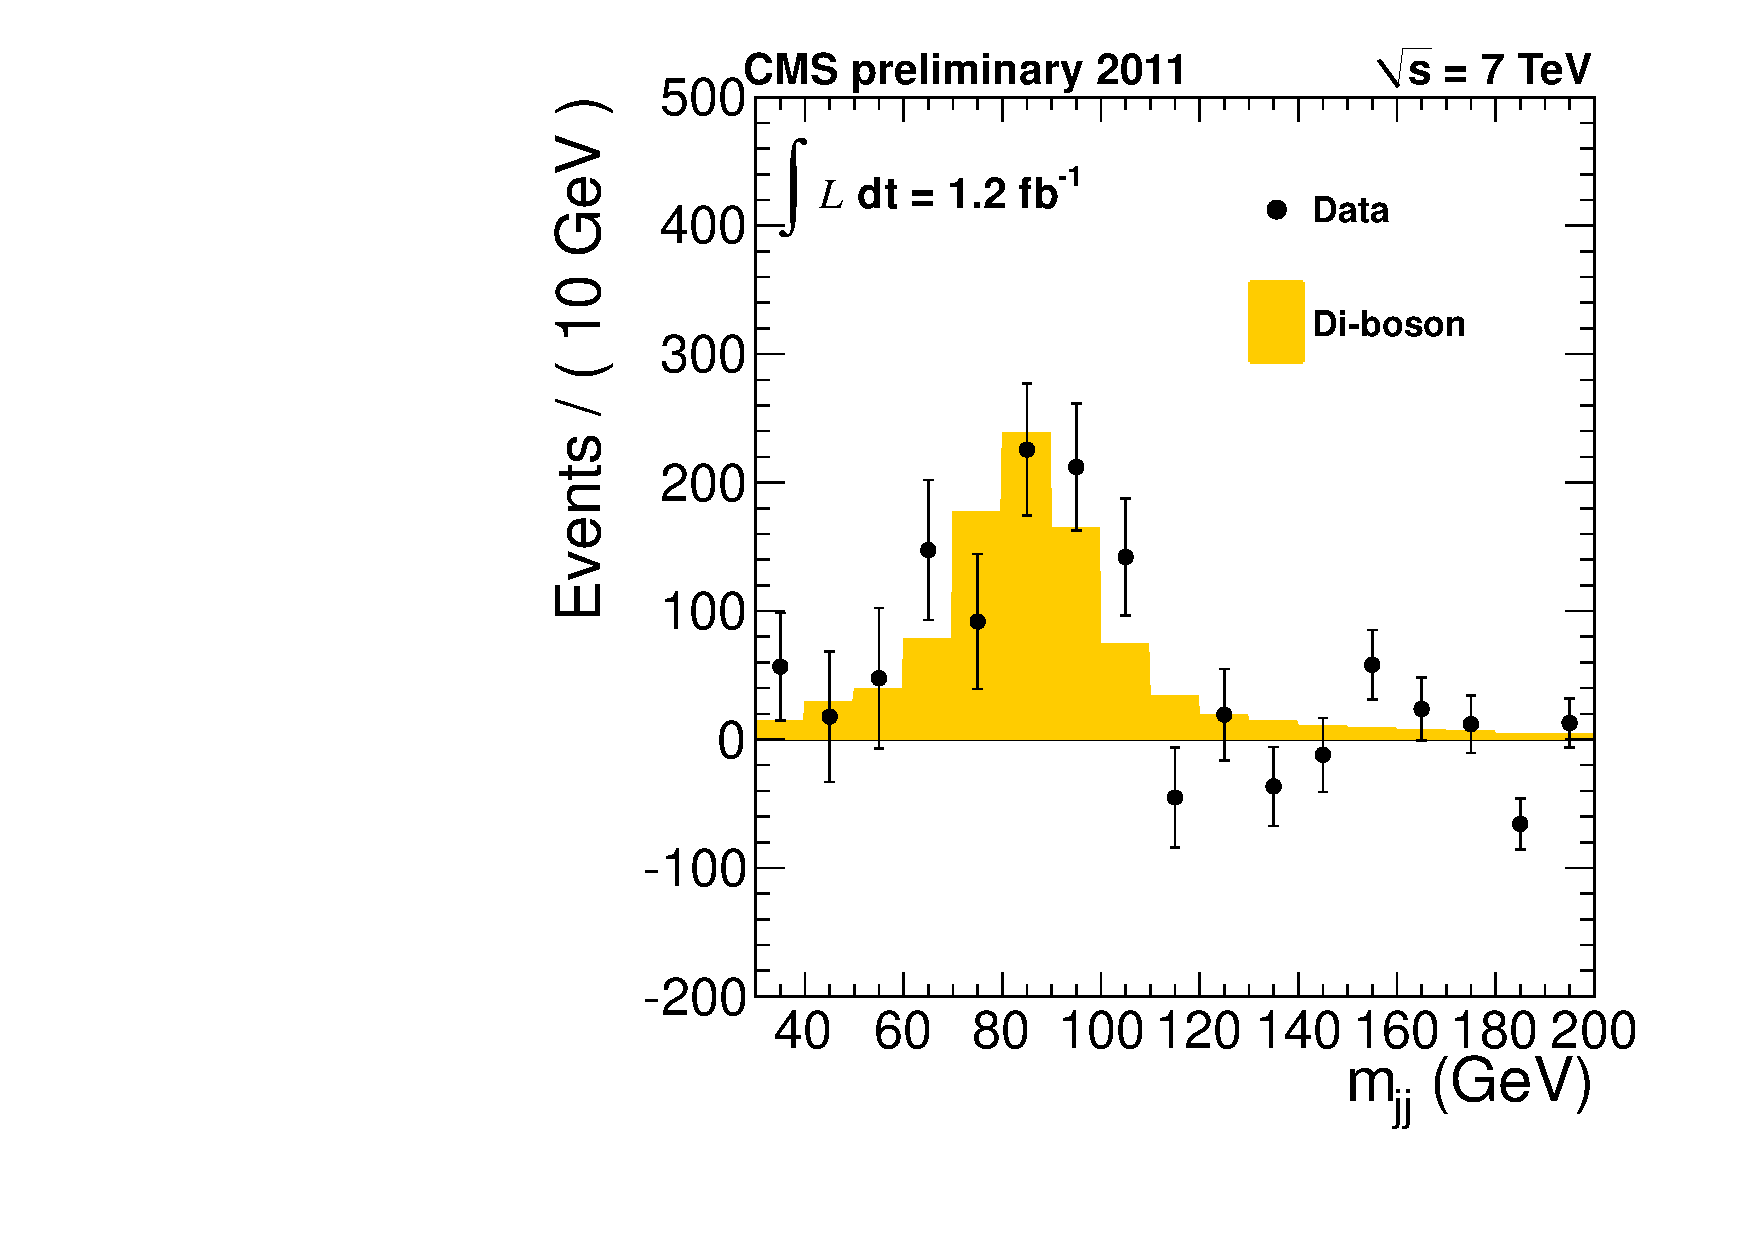
\includegraphics[width=0.48\textwidth]{figs/J2pTomjj_mJJ-combined-fit-subtracted.pdf}
\put(-0.80,0.0){(b)} 
\caption{Fit results with the $Jet2_{p_T}/m_{jj}>0.3$ cut before (a)
and after (b) the subtraction of the background components.}
\label{fig:J2pTomjjCutFit}}
\end{figure}
%%%%%%%
\clearpage
\section{Analysis using CDF-like cuts and progressively tighter cuts}
We further examine fit configurations by gradually changing the cuts
from CDF-like to the ones used for measuring the WW$\to l\nu jj$
cross-section. Specifically, we examine the following five stages:
\begin{itemize}
\item CDF-like (aka Standard) cuts
\item Kinematic Fit $\chi^2/NDF<10.0$ (not used in generic Mjj analysis)
\item $-0.6<\cos (\textrm{JacksonAngle})<0.8$ (not used in generic Mjj analysis)
\item $Jet2_{p_T}/m_{jj}>0.3$
\item Anti-$b$-tag (medium, highefficiency, Simple Secondary Vertex) both jets
\end{itemize}
The impact is shown in Figure~\ref{fig:CDFtoWWcuts} and summarized in
Table~\ref{table:CDFtoWWcuts}. As expected, the fit quality improves
with additional cuts, while the WW Peak becomes more well-defined and
pronounced. The residual fluctuations are consistent with 0.

\begin{table}[tb]
\caption{Transition from CDF-like to Diboson Analysis cuts.}
\begin{center}
\begin{tabular}{|c|c|c|c|}
\hline
   Cut                           & WW yield     & W$jj$ yield    & $S/B$   \cr \hline
\vspace{-0.5cm} & & \cr
{CDF-like}                       & $903\pm 204$ & $29291\pm 269$ & $0.031$ \cr \hline
{$\chi^2/NDF<10.0$}              & $806\pm 213$ & $24117\pm 267$ & $0.033$ \cr \hline
{$-0.6<\cos (JacksonAngle)<0.8$} & $800\pm 211$ & $22468\pm 255$ & $0.036$ \cr \hline
{$Jet2_{p_T}/m_{jj}>0.3$}        & $847\pm 228$ & $20557\pm 272$ & $0.041$ \cr \hline
{anti-$b$-tag}                   & $964\pm 213$ & $18672\pm 254$ & $0.052$ \cr \hline
\end{tabular}
\end{center}
\label{table:CDFtoWWcuts}
\end{table}
%%%%%%%%%%%%%%%%%%%%%%%%%%%%
%%%%%%%
\begin{figure}[h!] {\centering
\unitlength=0.33\linewidth
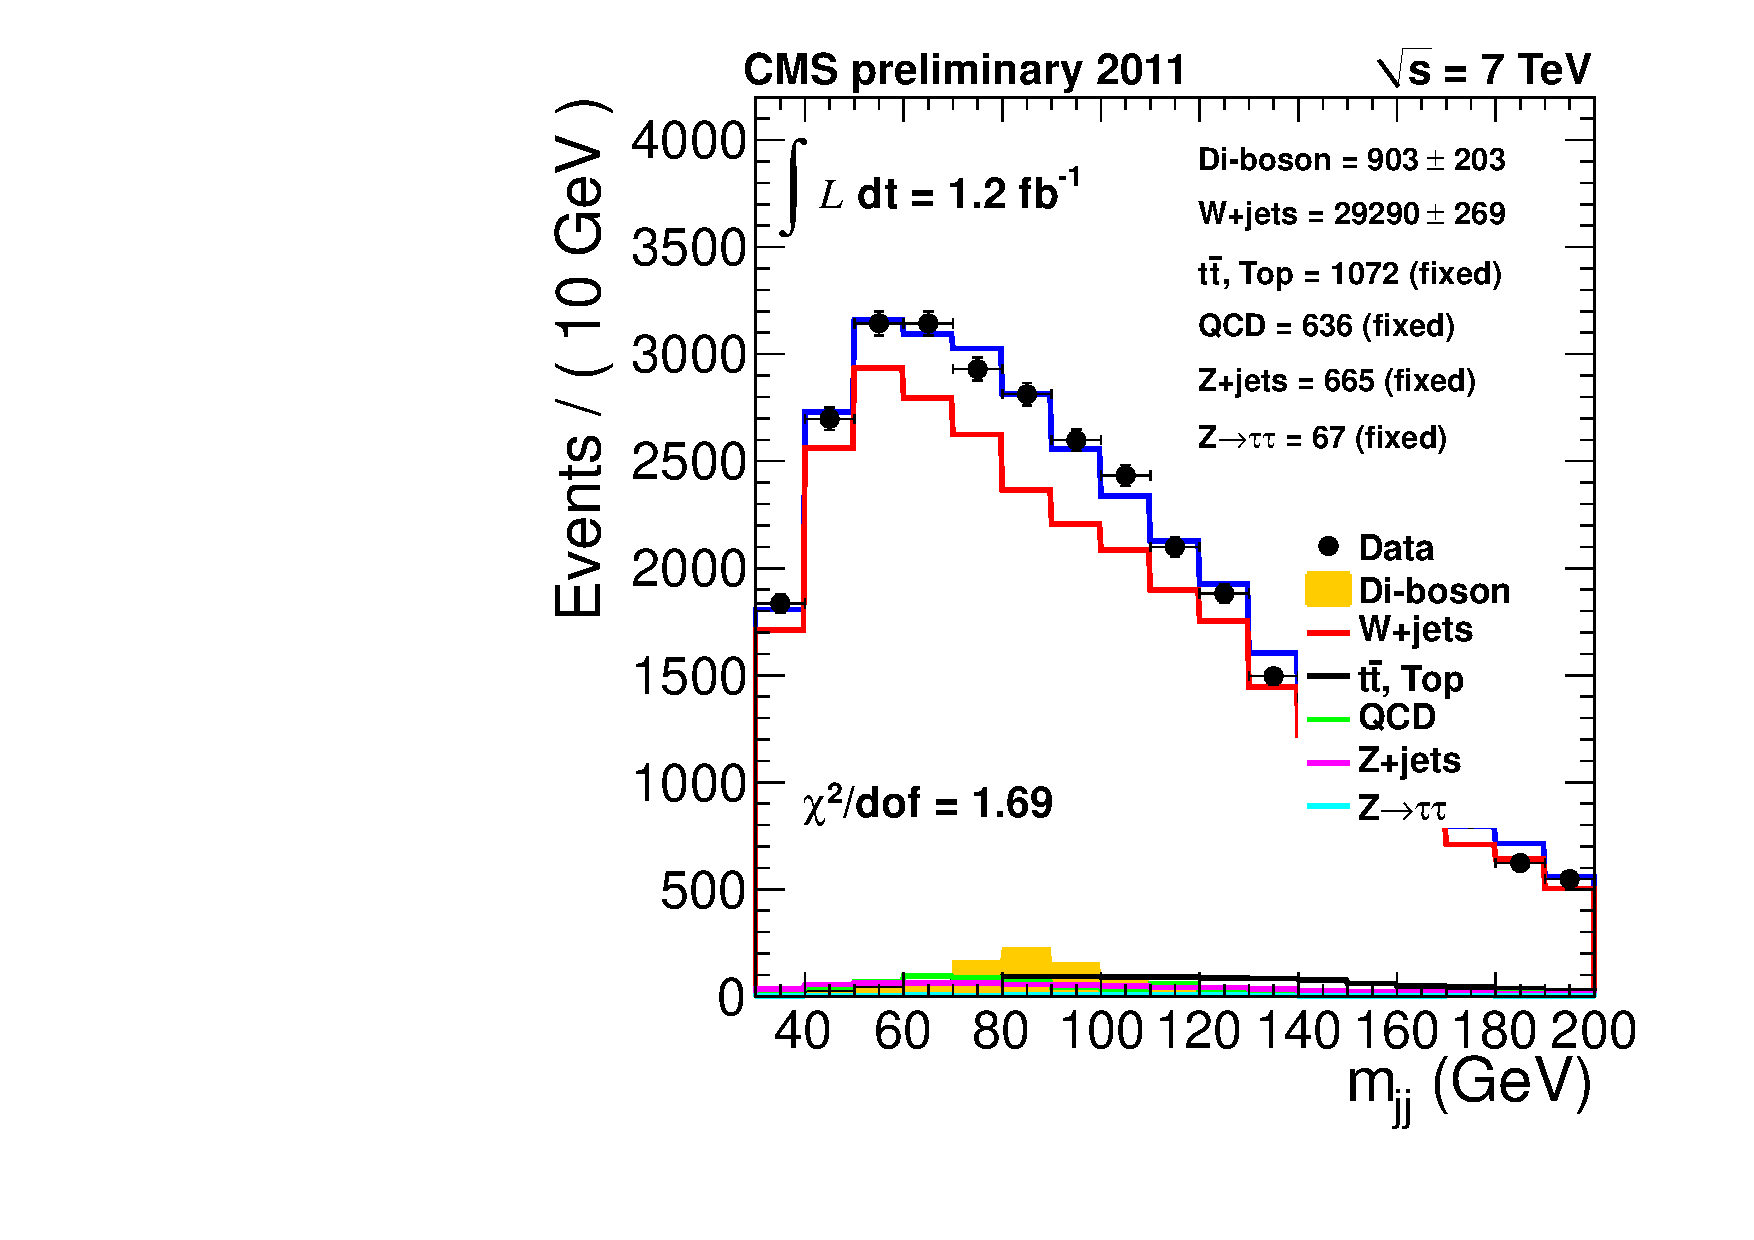
\includegraphics[width=0.31\textwidth]{figs/CDFtoWW_s0_mJJ-combined-fit.pdf} 
\unitlength=0.33\linewidth
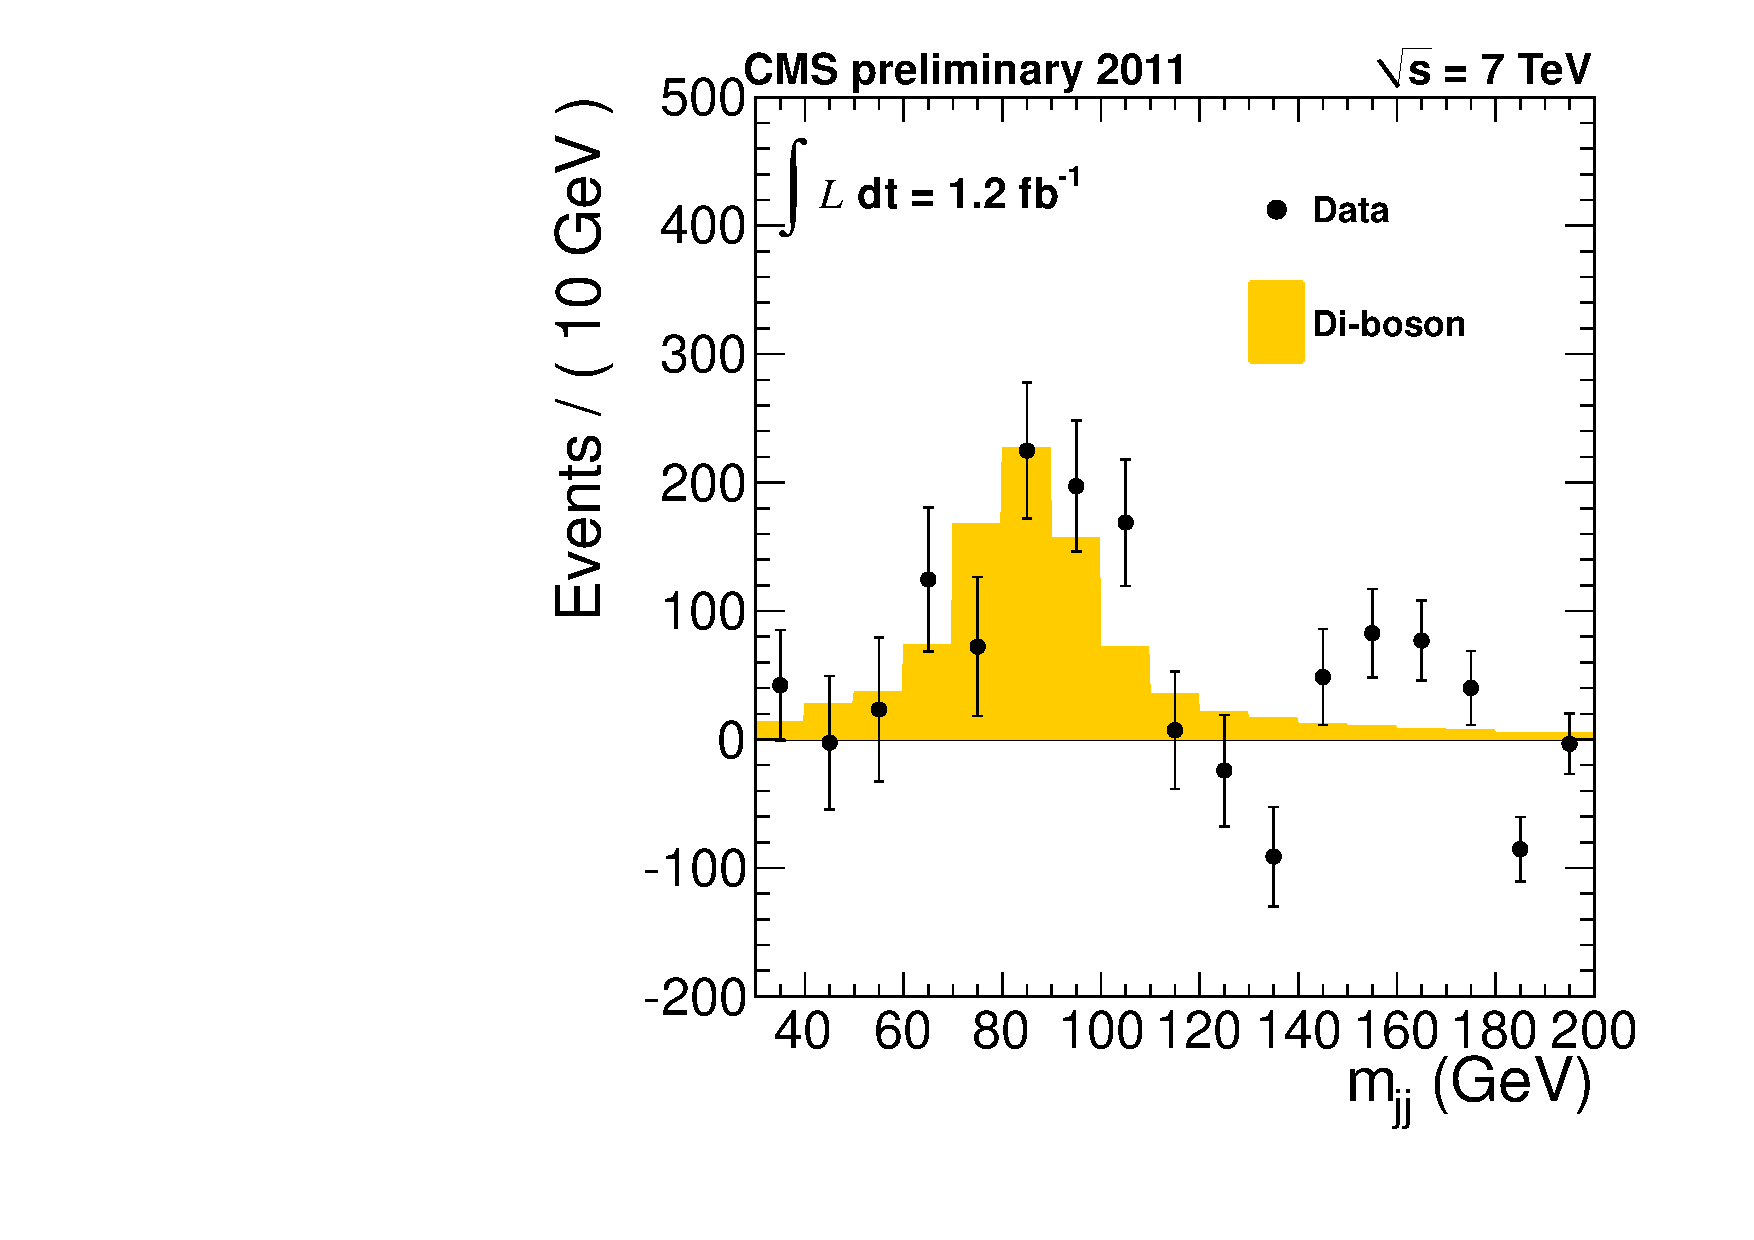
\includegraphics[width=0.31\textwidth]{figs/CDFtoWW_s0_mJJ-combined-fit-subtracted.pdf} 
\unitlength=0.33\linewidth
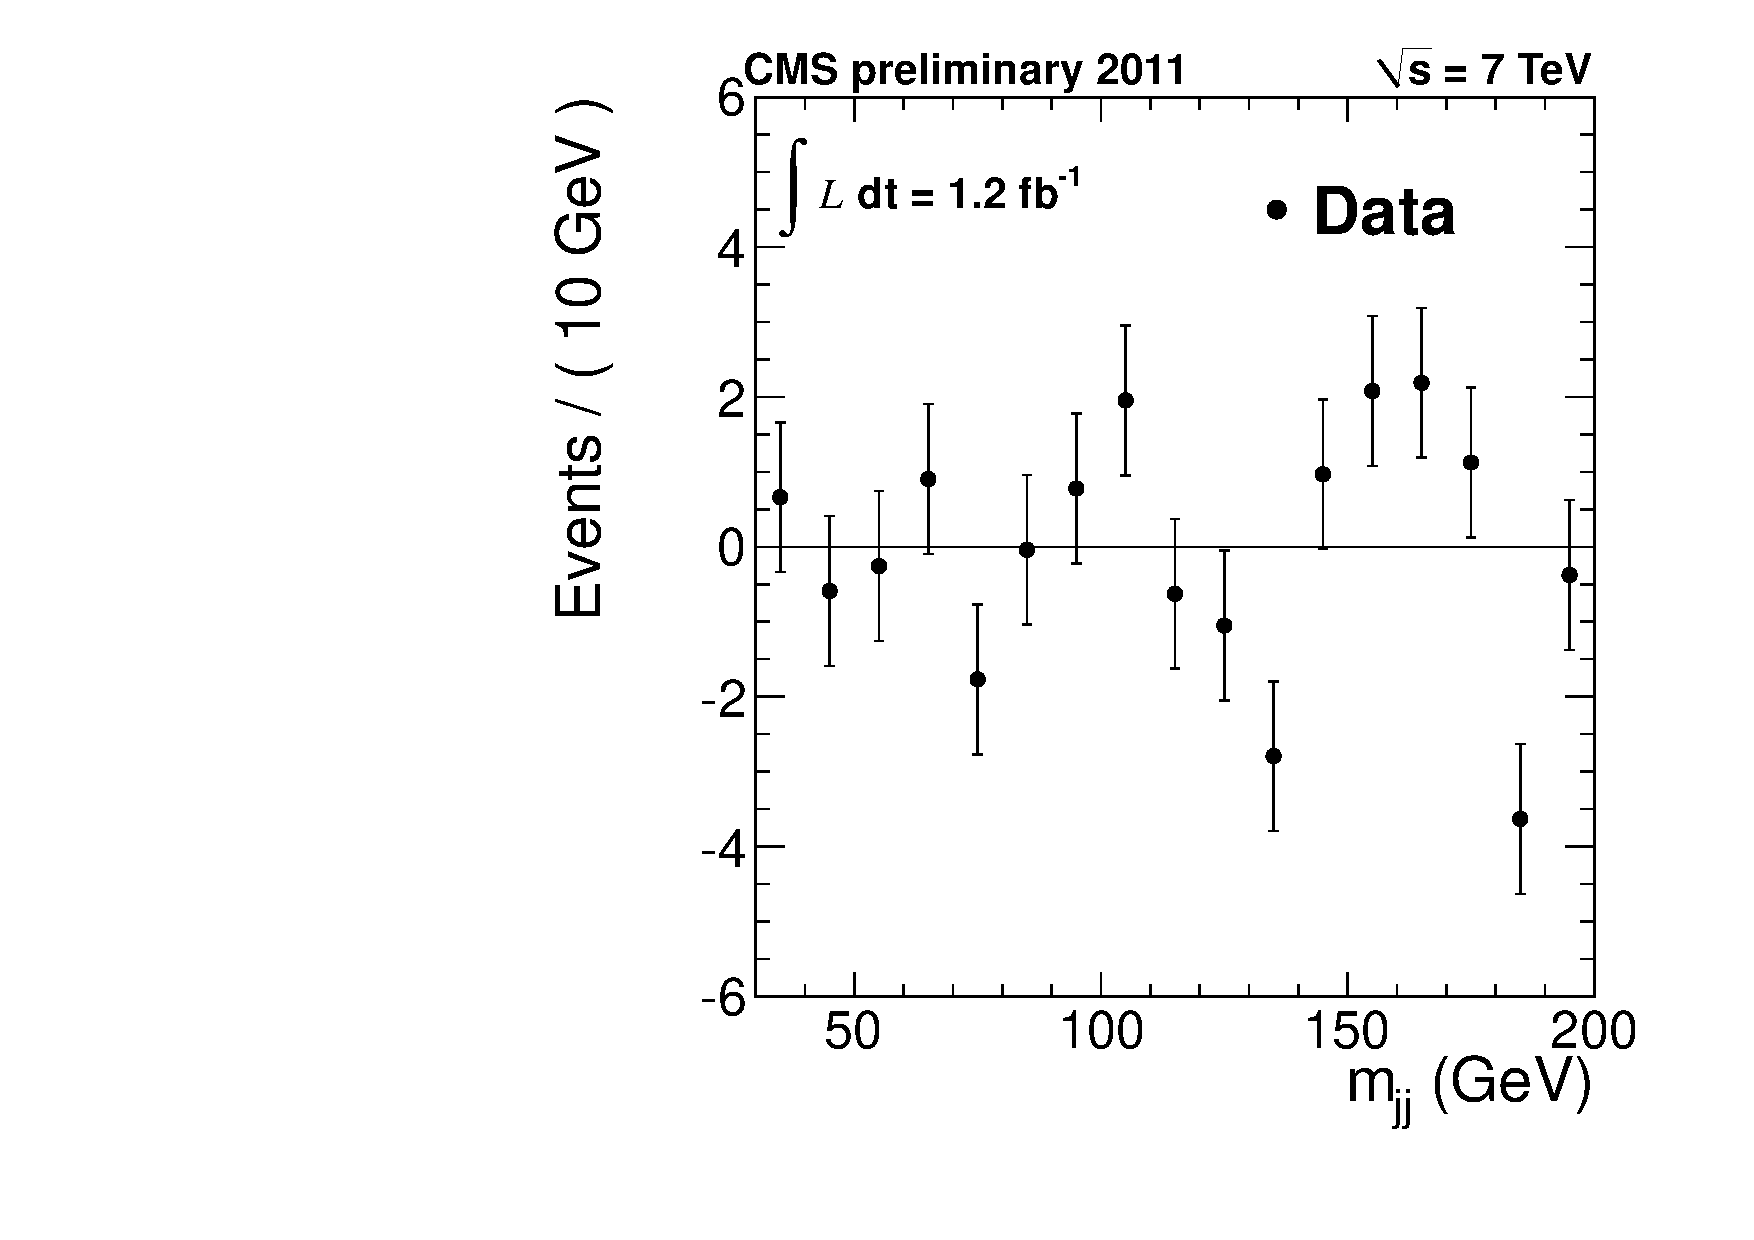
\includegraphics[width=0.31\textwidth]{figs/CDFtoWW_s0_mJJ-combined-fit-residual.pdf} \\
%%\put(-0.50,0.0){a)} \\
\unitlength=0.33\linewidth
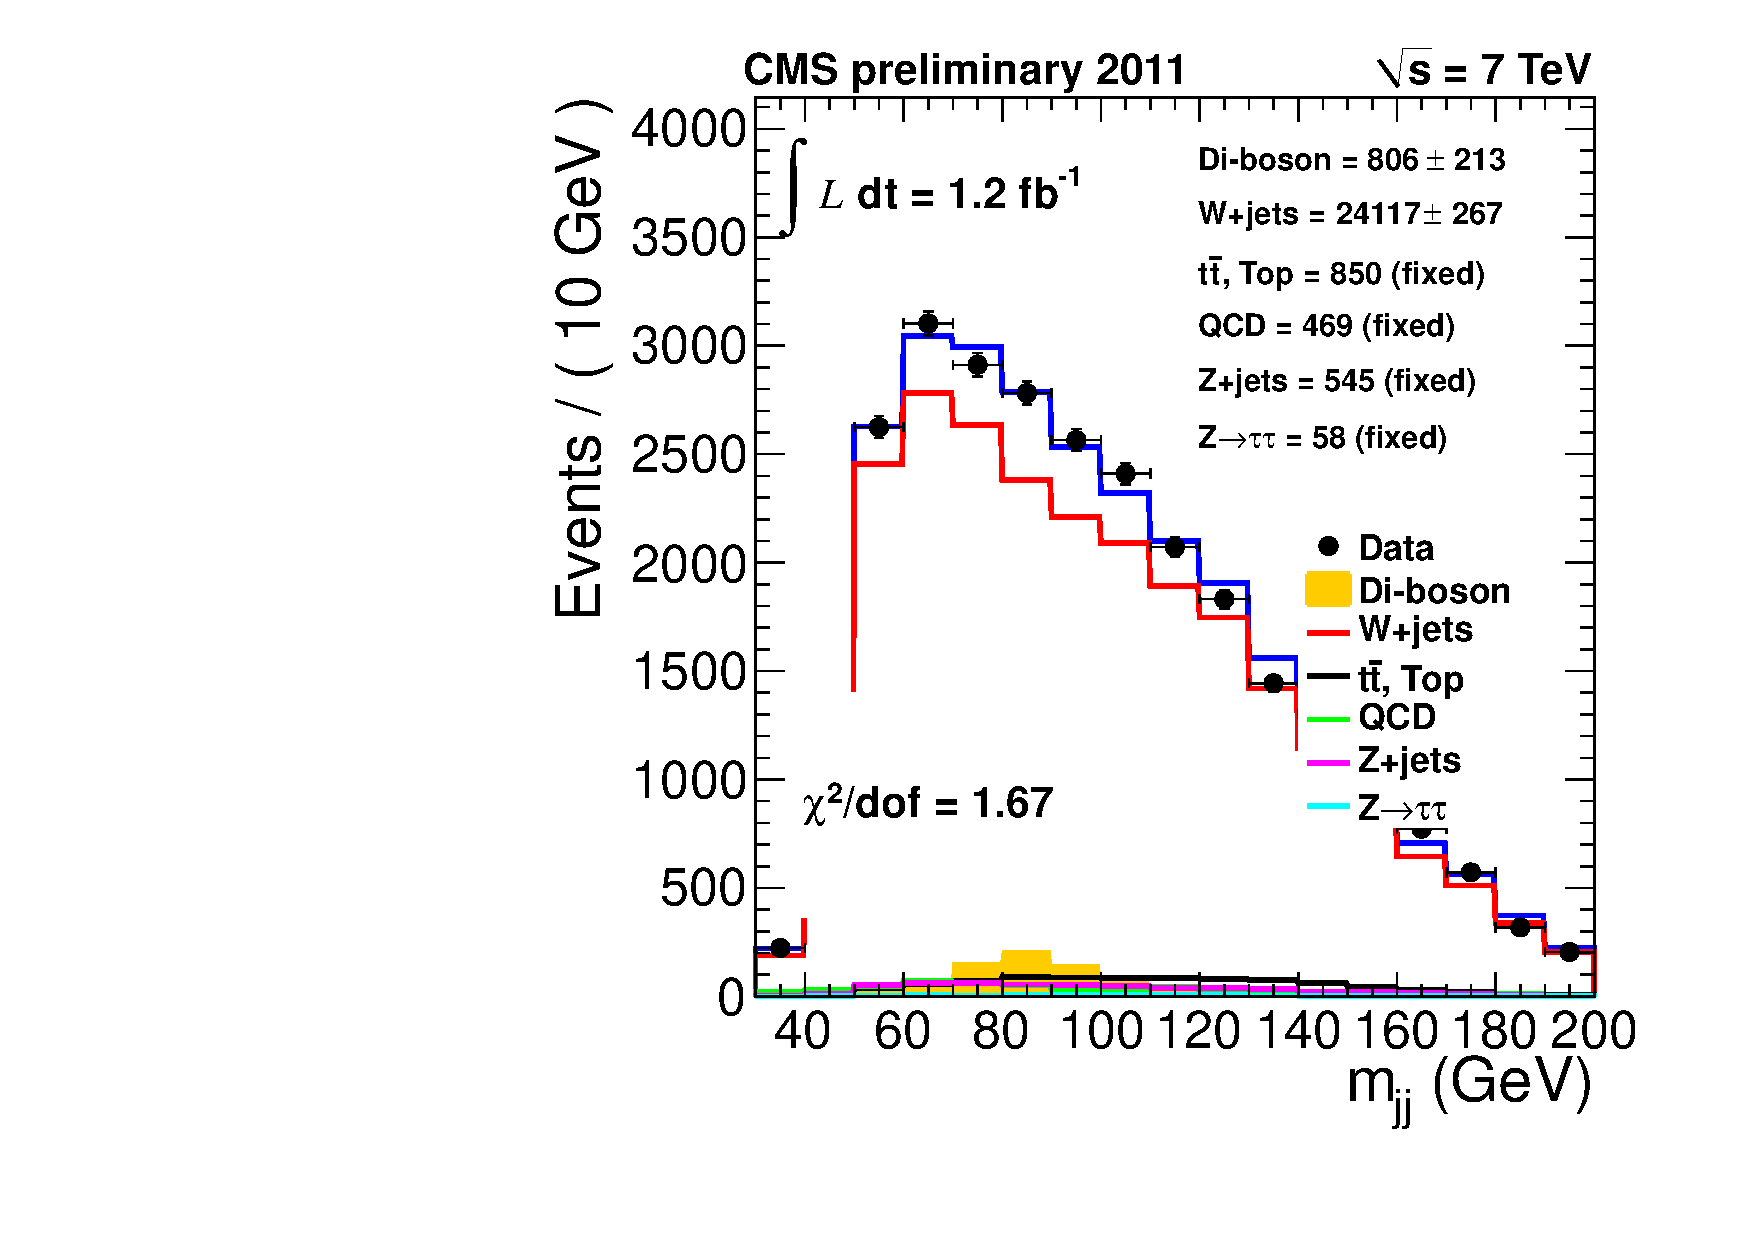
\includegraphics[width=0.31\textwidth]{figs/CDFtoWW_s1_mJJ-combined-fit.pdf} 
\unitlength=0.33\linewidth
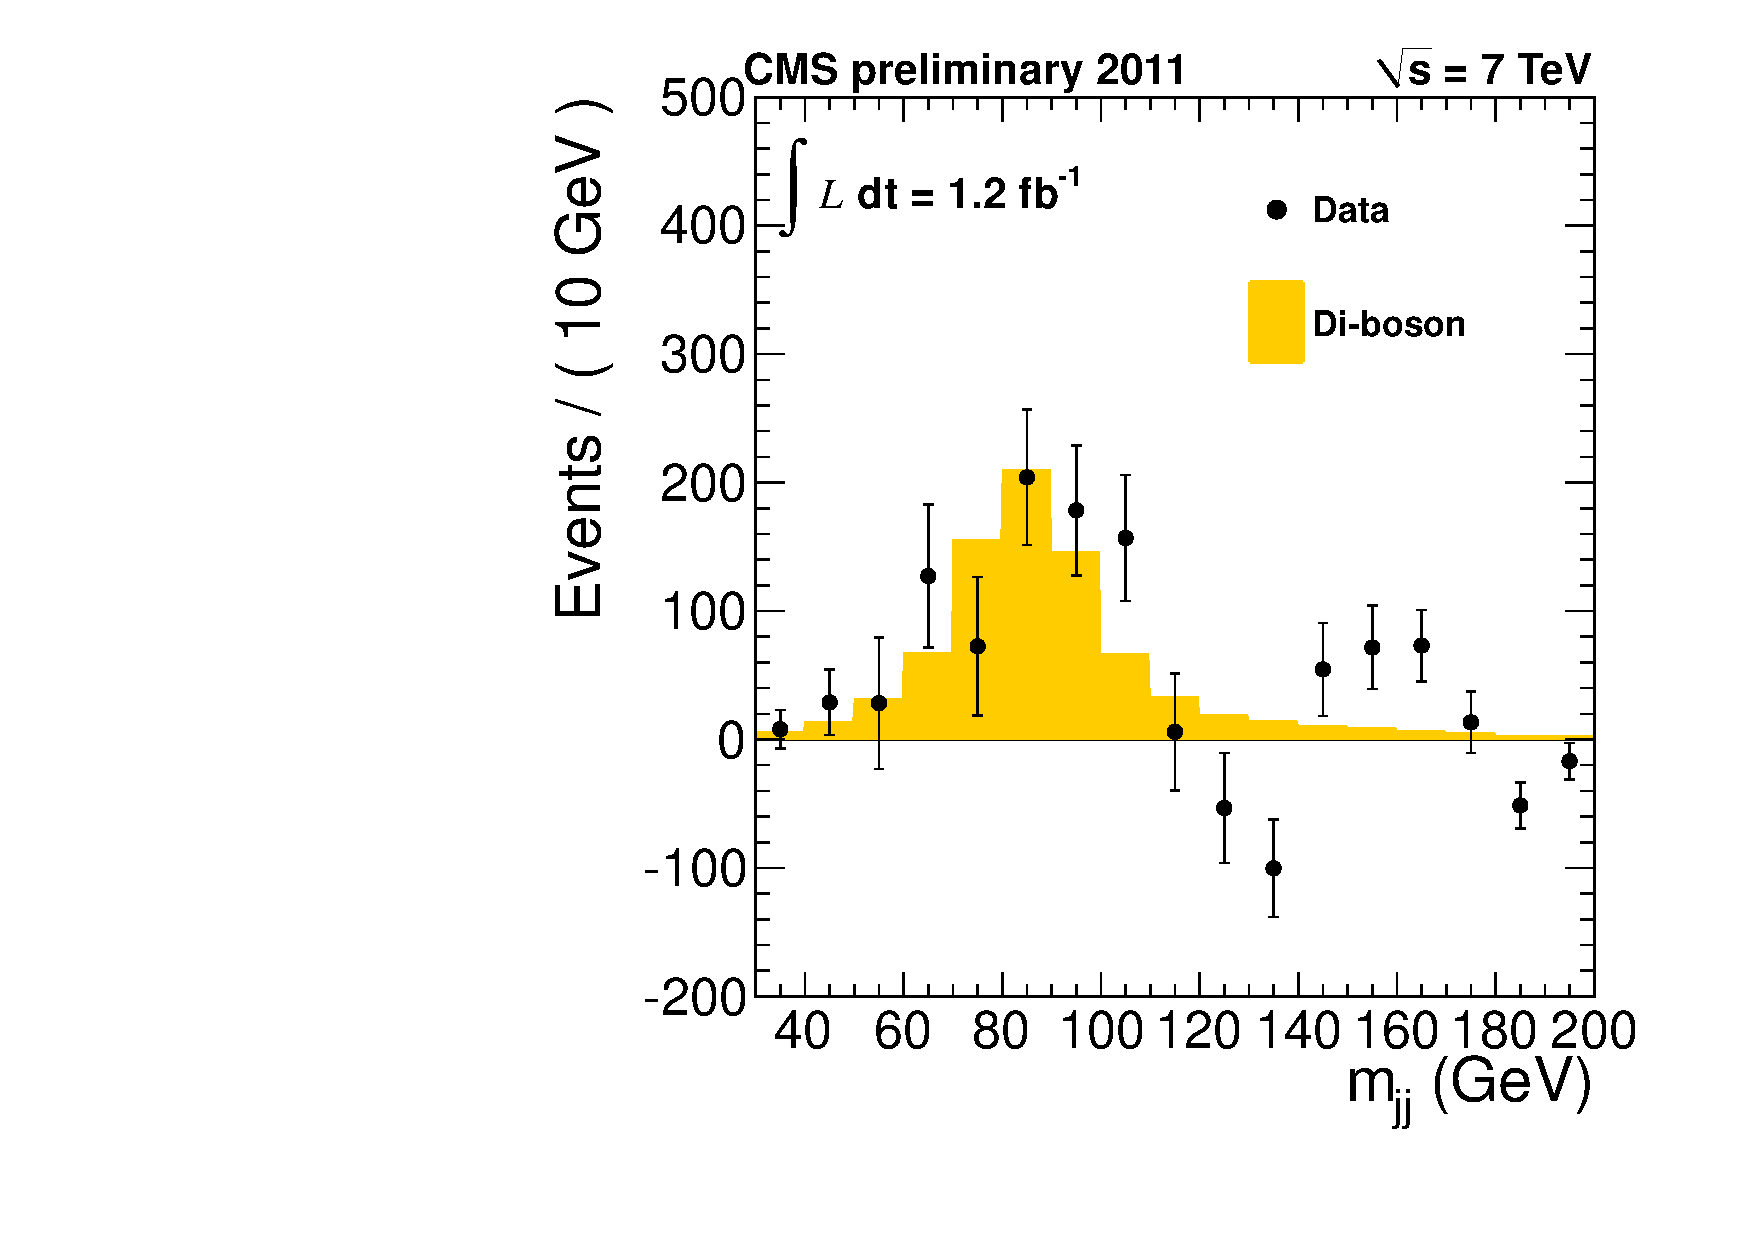
\includegraphics[width=0.31\textwidth]{figs/CDFtoWW_s1_mJJ-combined-fit-subtracted.pdf} 
\unitlength=0.33\linewidth
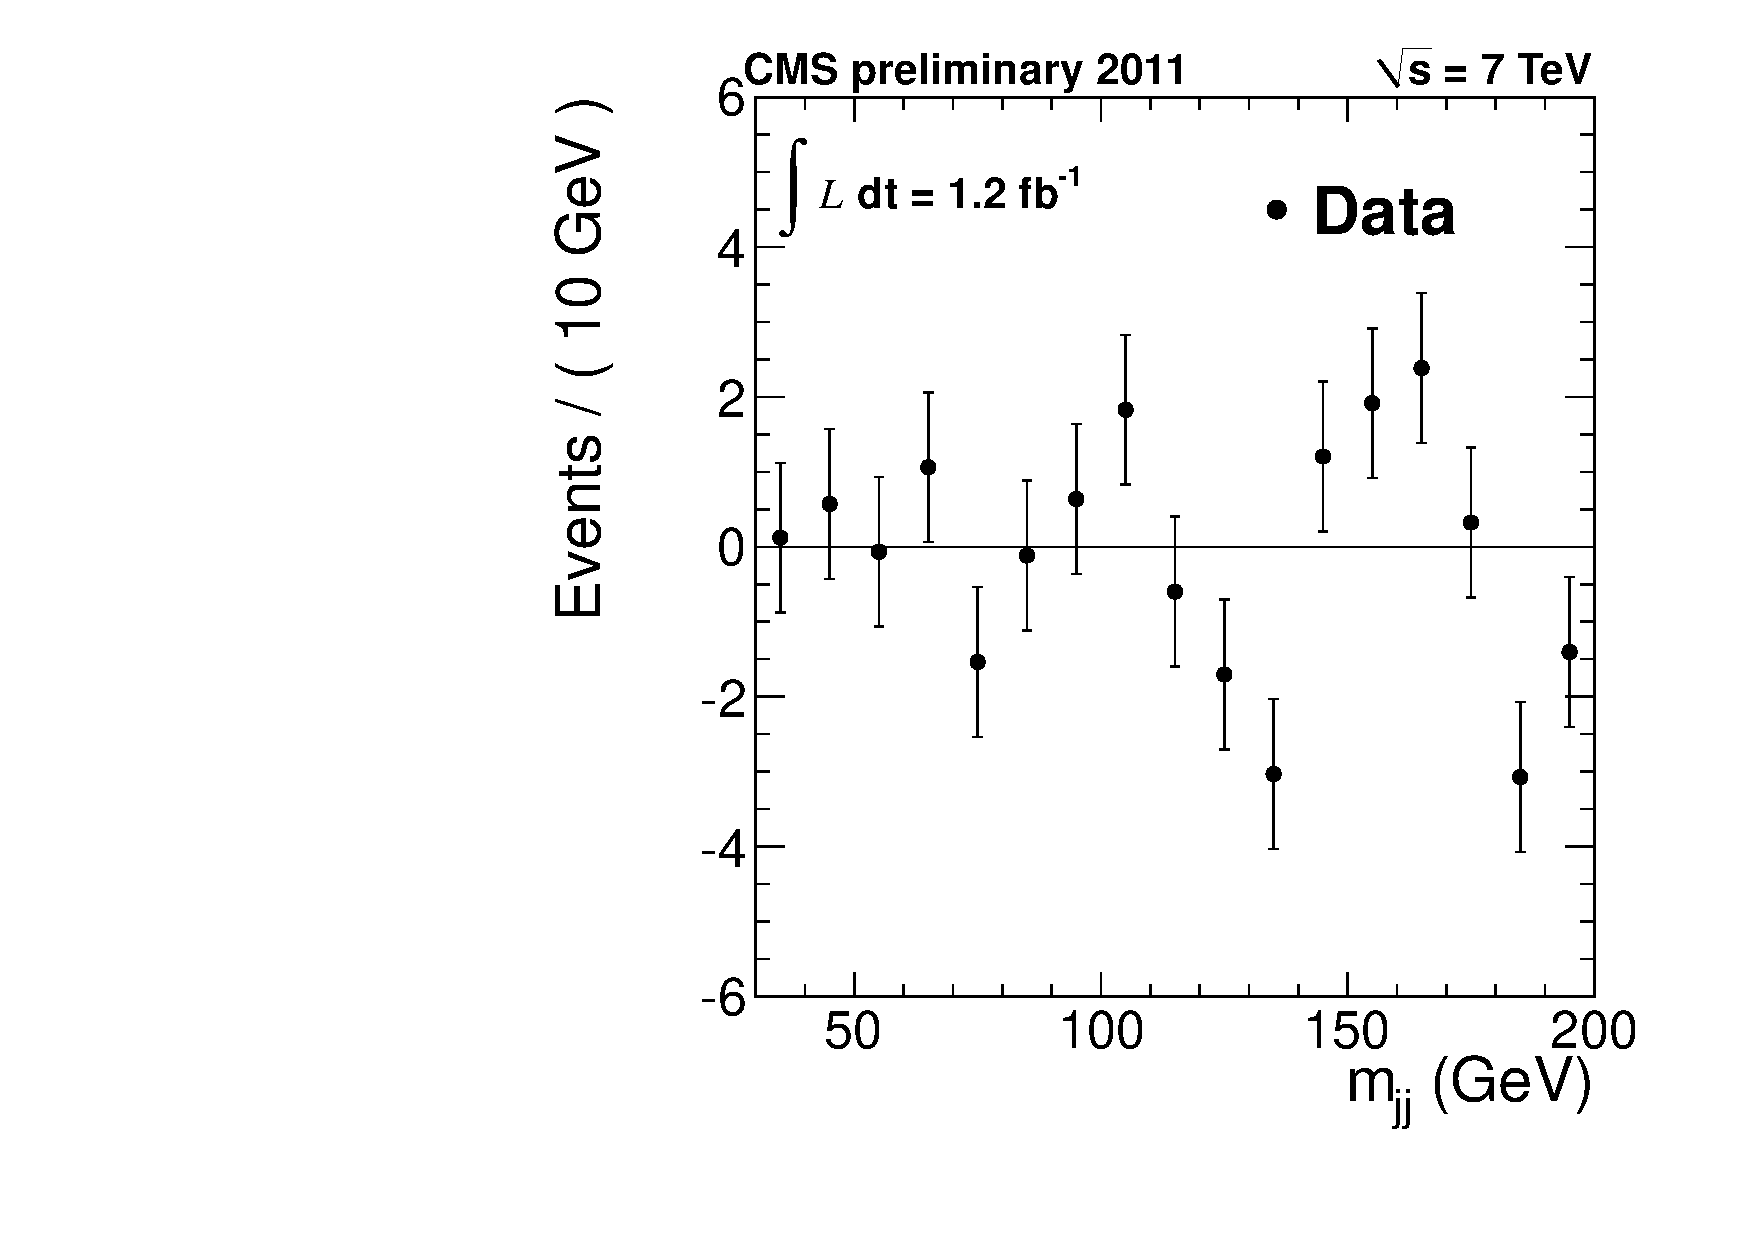
\includegraphics[width=0.31\textwidth]{figs/CDFtoWW_s1_mJJ-combined-fit-residual.pdf} \\
%%\put(-0.50,0.0){b)} \\
\unitlength=0.33\linewidth
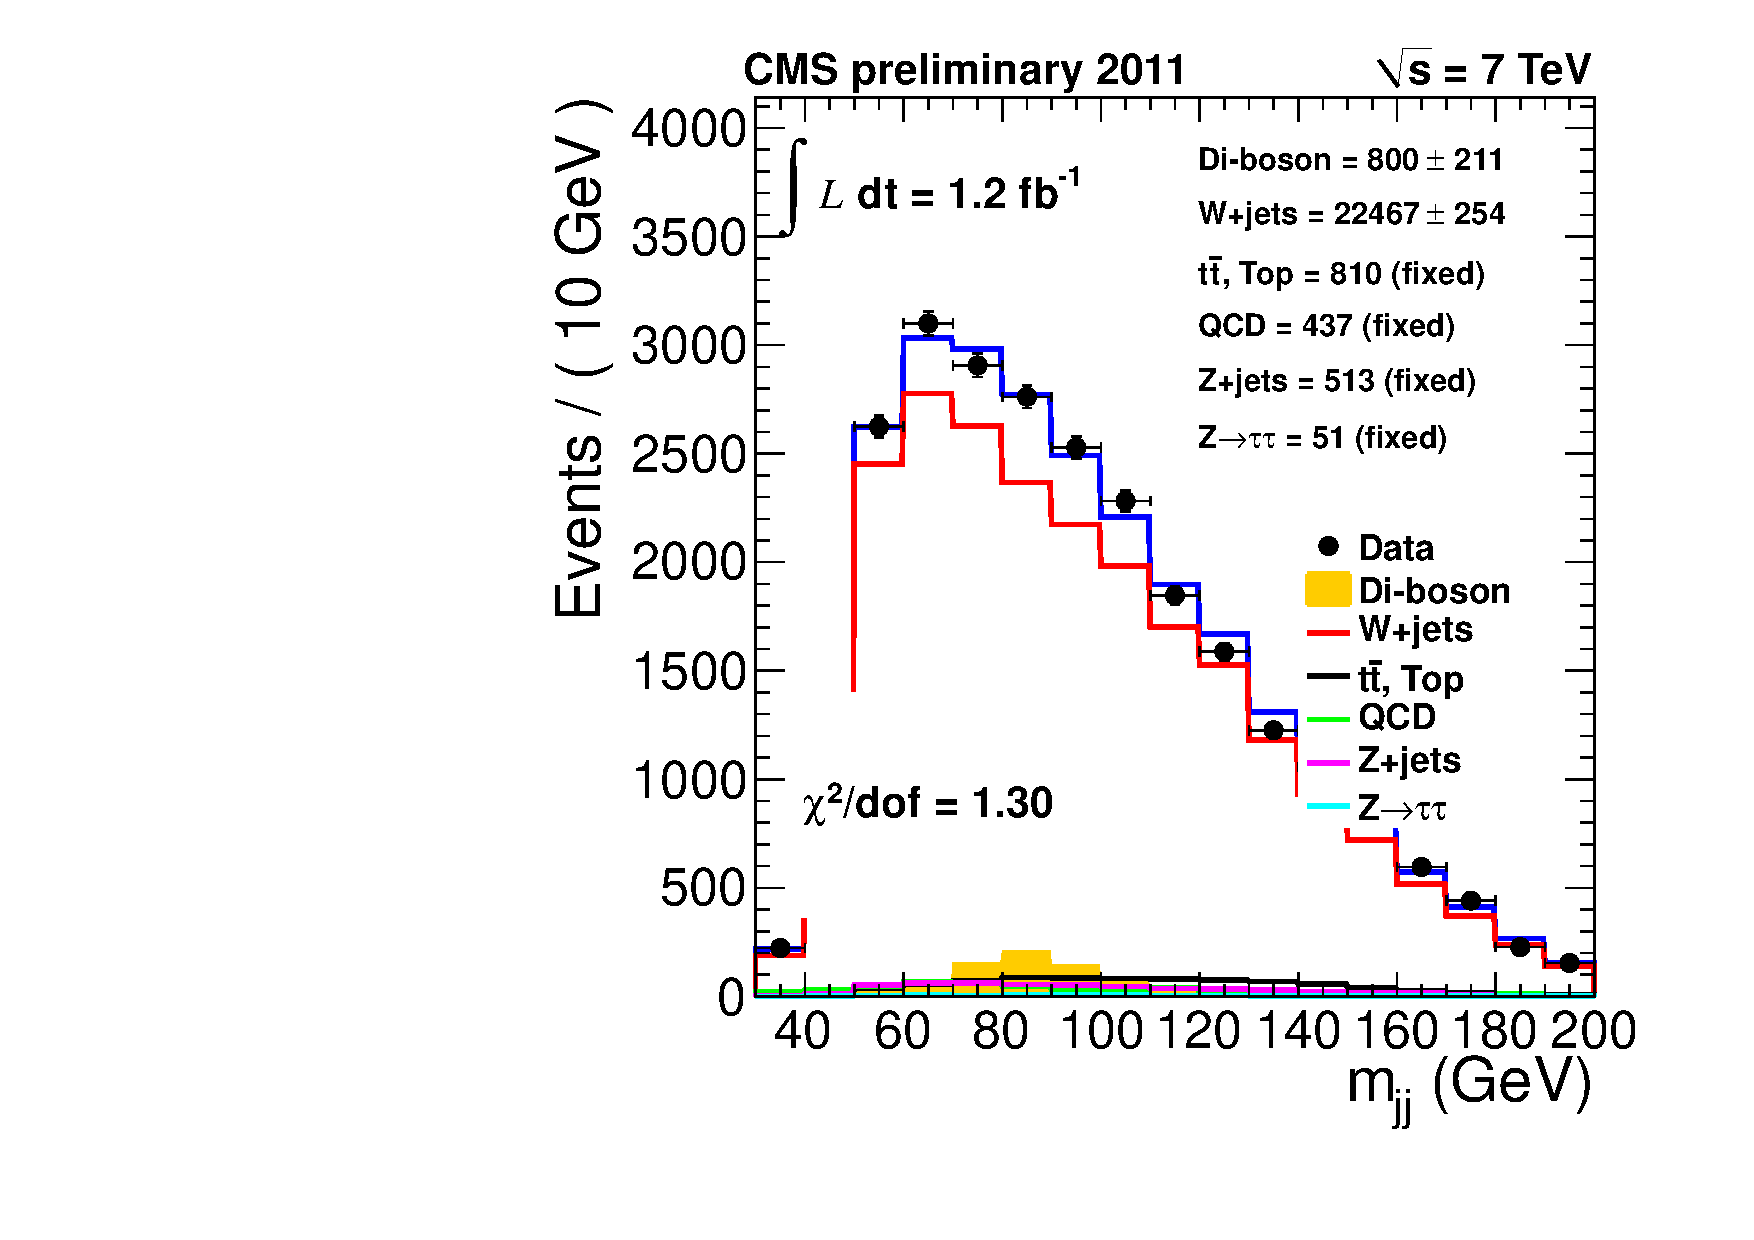
\includegraphics[width=0.31\textwidth]{figs/CDFtoWW_s2_mJJ-combined-fit.pdf} 
\unitlength=0.33\linewidth
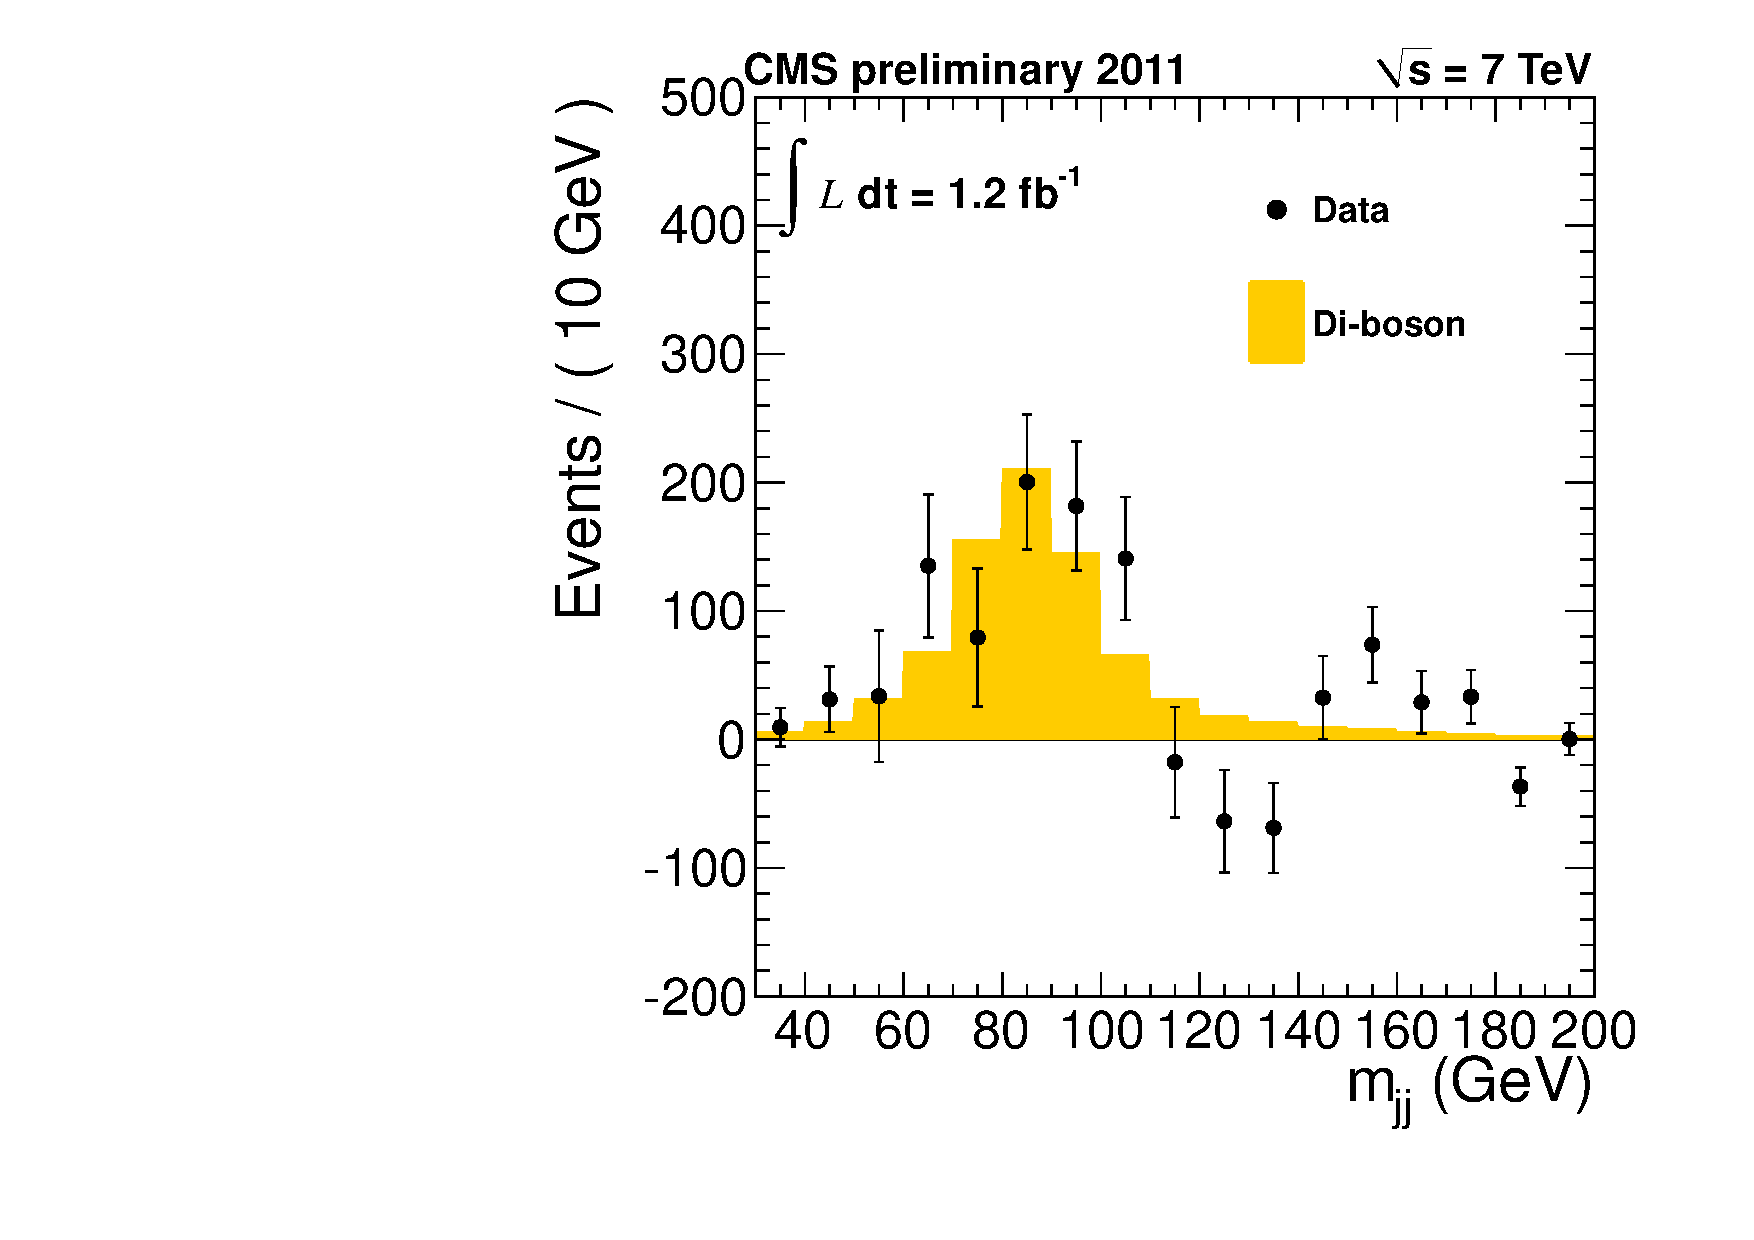
\includegraphics[width=0.31\textwidth]{figs/CDFtoWW_s2_mJJ-combined-fit-subtracted.pdf} 
\unitlength=0.33\linewidth
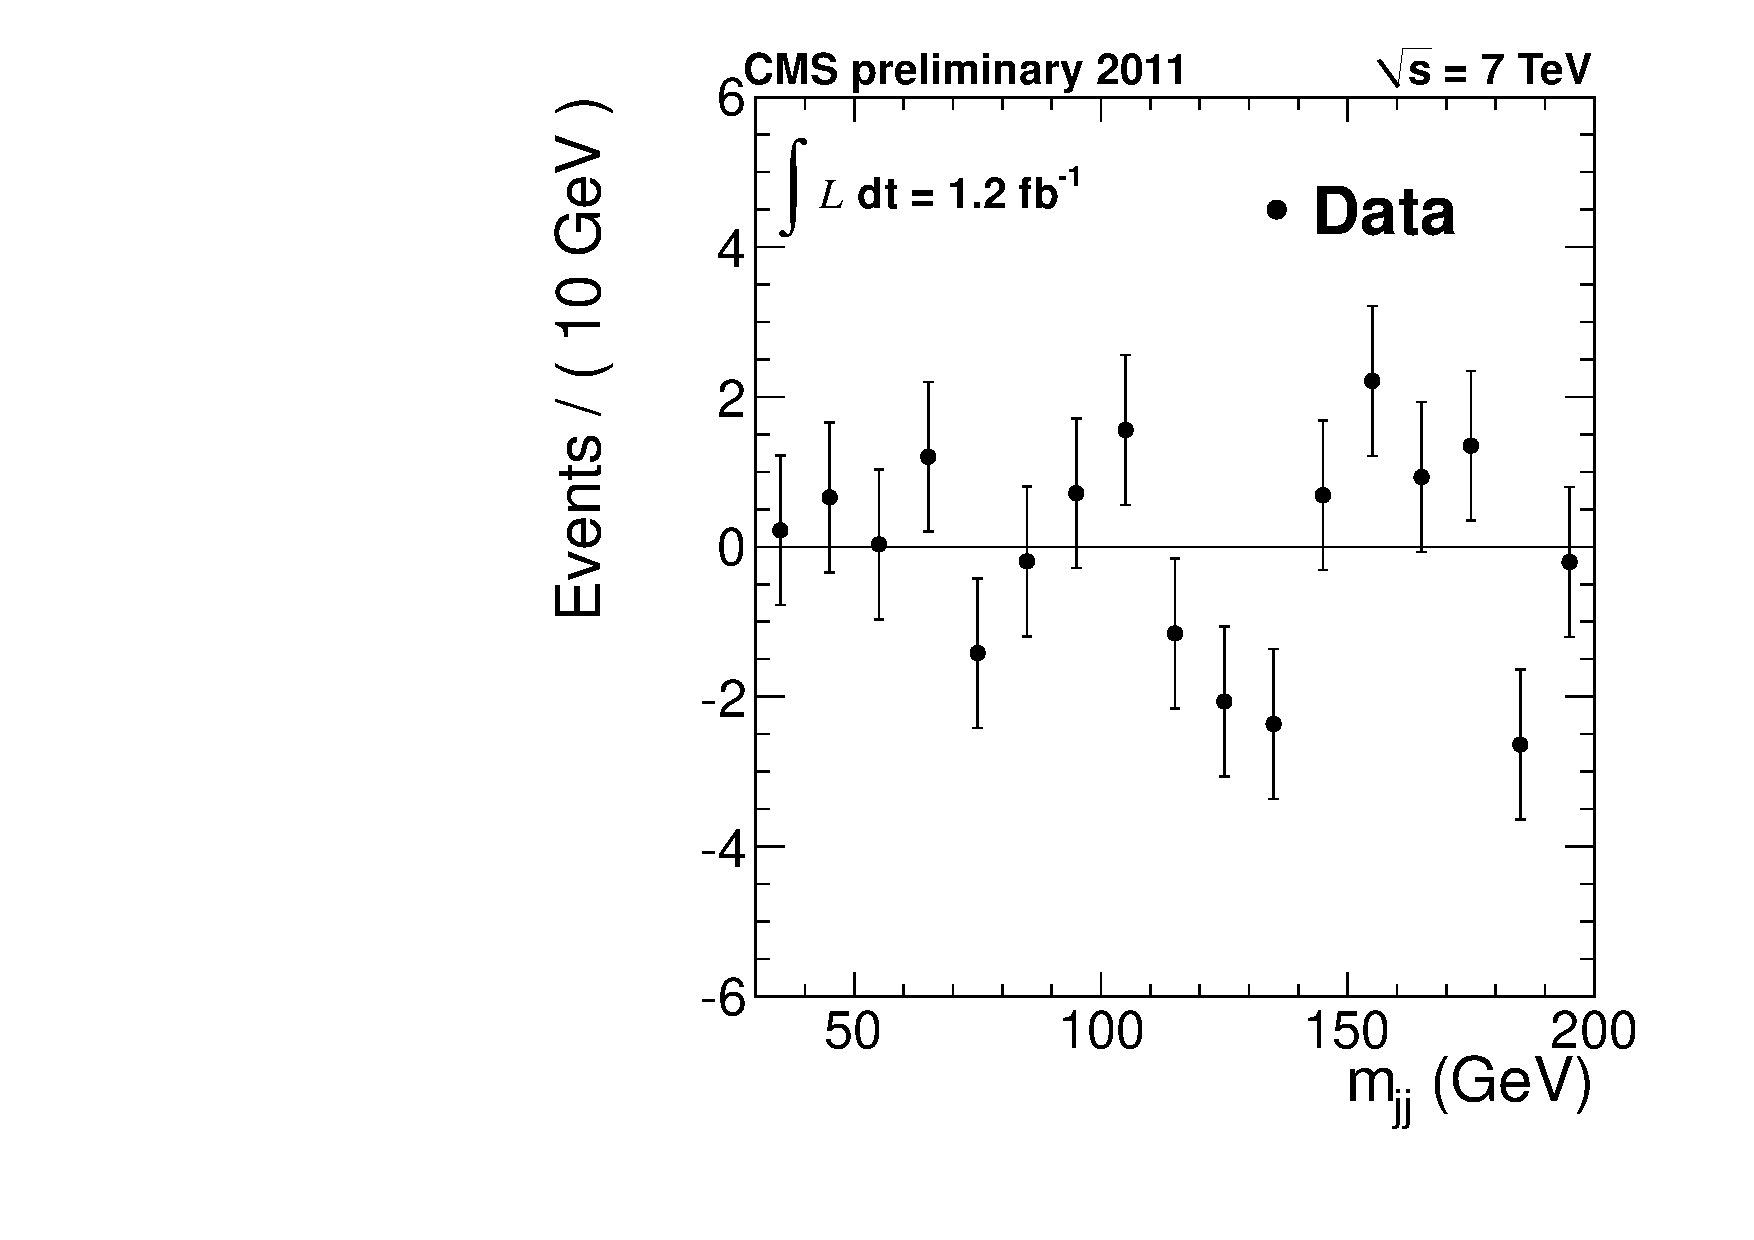
\includegraphics[width=0.31\textwidth]{figs/CDFtoWW_s2_mJJ-combined-fit-residual.pdf} \\
%%\put(-0.50,0.0){c)} \\
\unitlength=0.33\linewidth
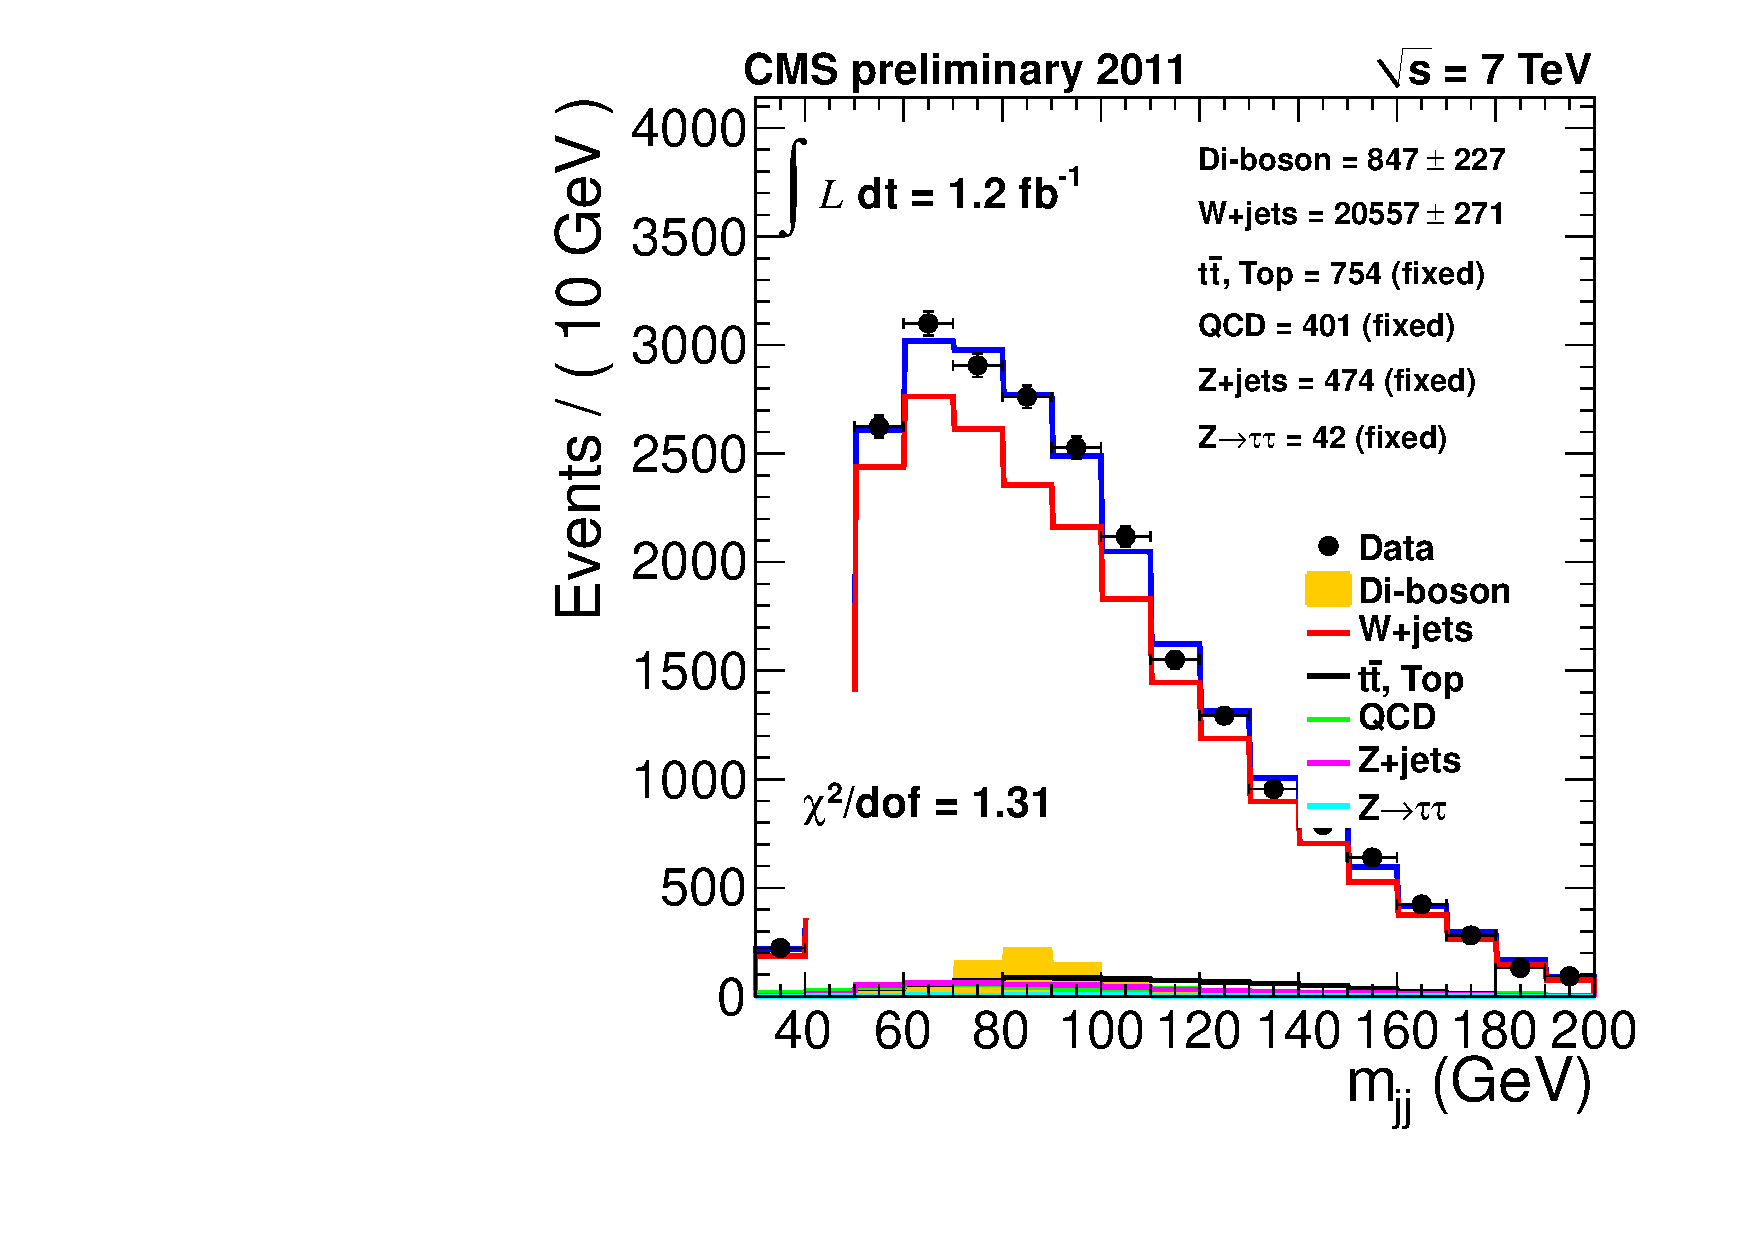
\includegraphics[width=0.31\textwidth]{figs/CDFtoWW_s3_mJJ-combined-fit.pdf} 
\unitlength=0.33\linewidth
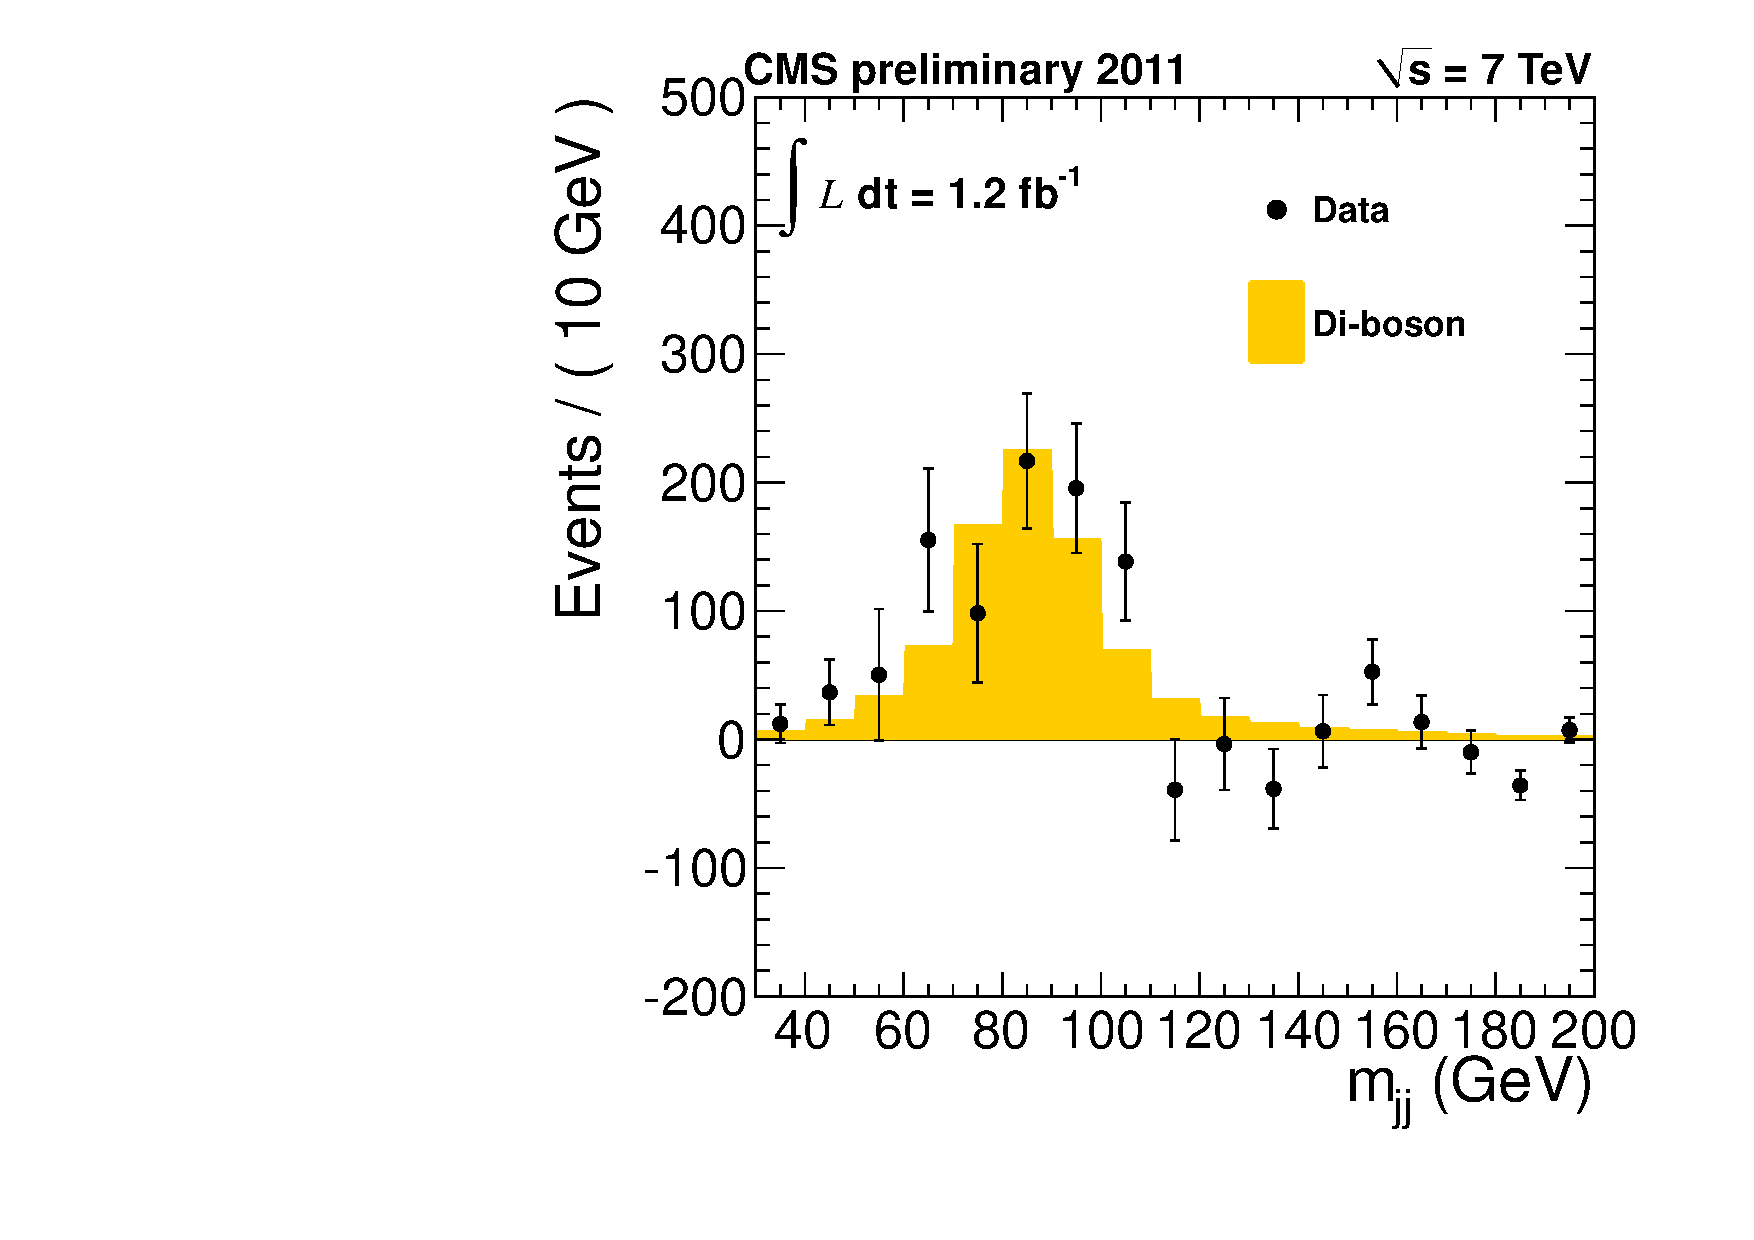
\includegraphics[width=0.31\textwidth]{figs/CDFtoWW_s3_mJJ-combined-fit-subtracted.pdf} 
\unitlength=0.33\linewidth
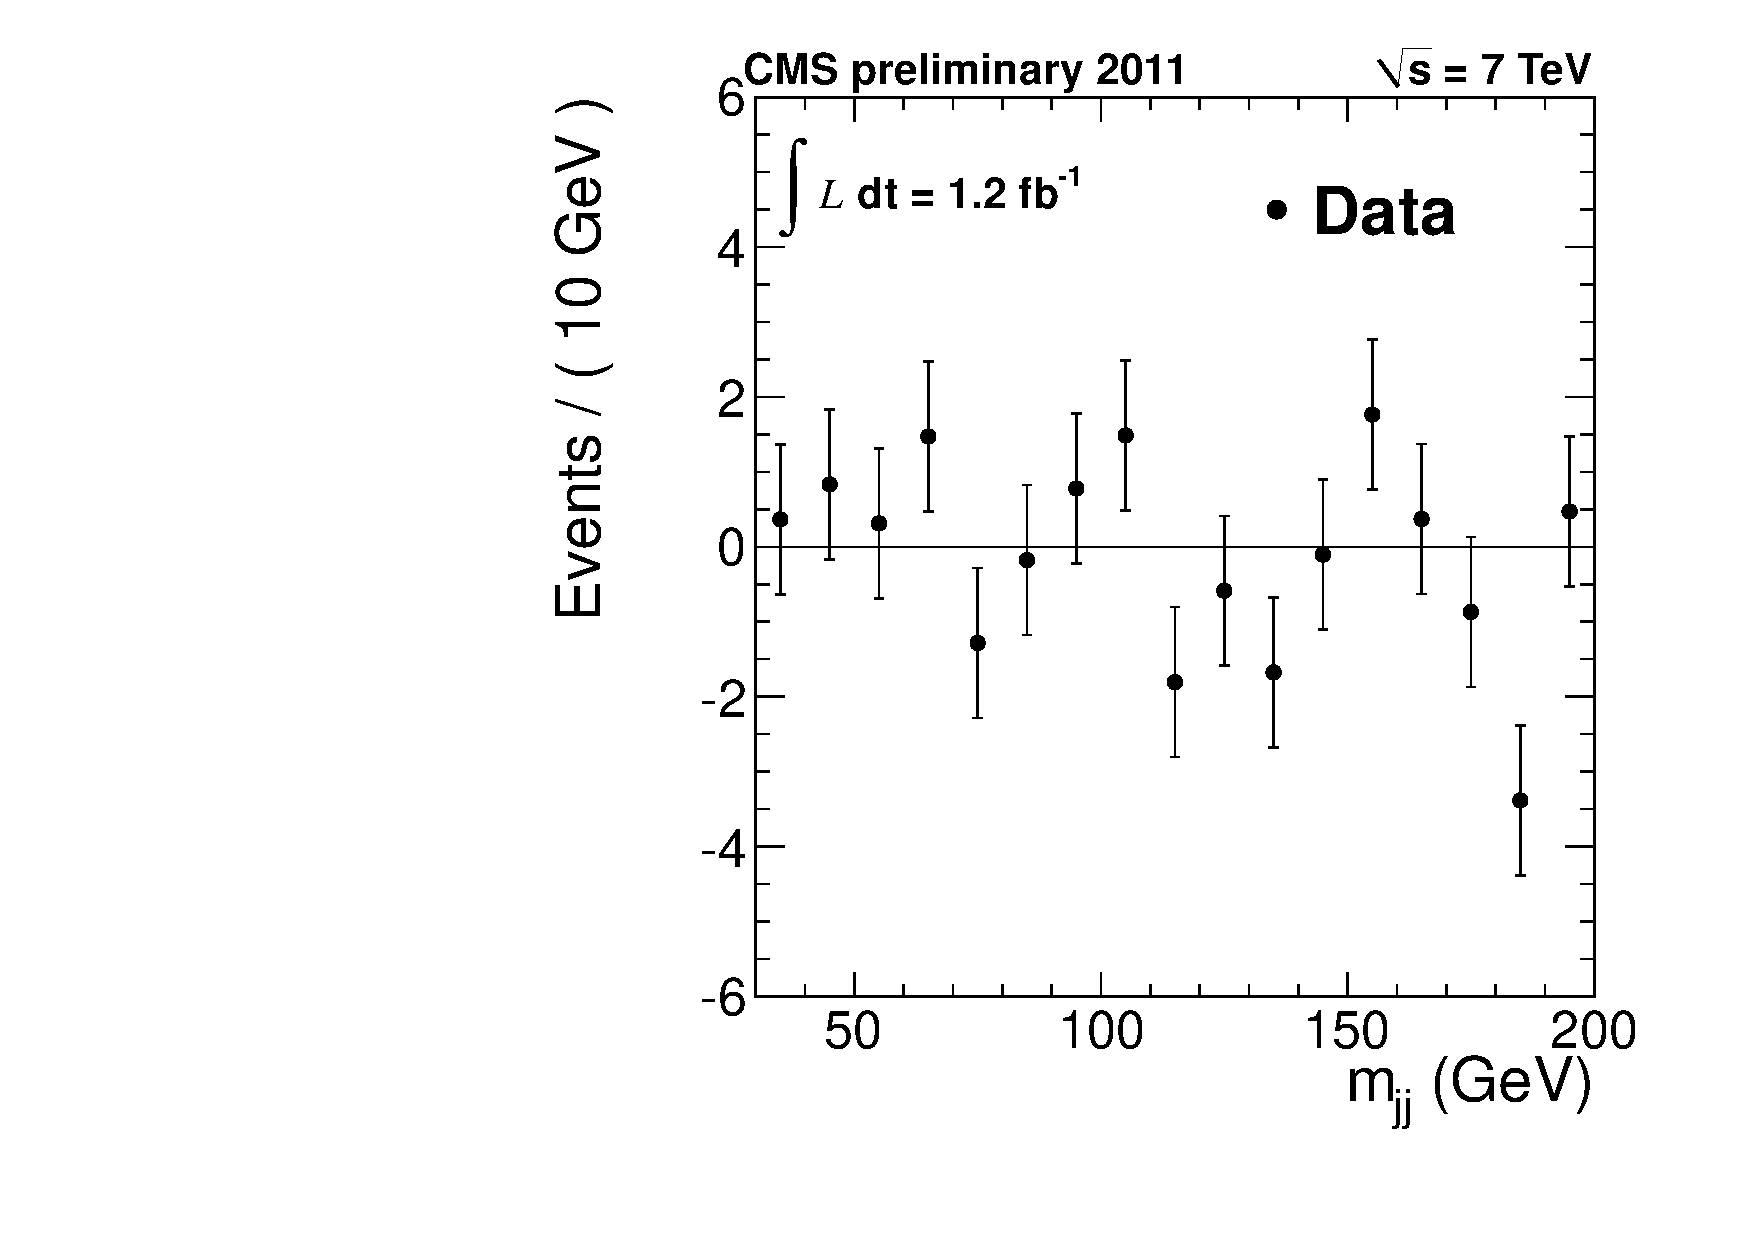
\includegraphics[width=0.31\textwidth]{figs/CDFtoWW_s3_mJJ-combined-fit-residual.pdf} \\
%%\put(-0.50,0.0){d)} \\
\unitlength=0.33\linewidth
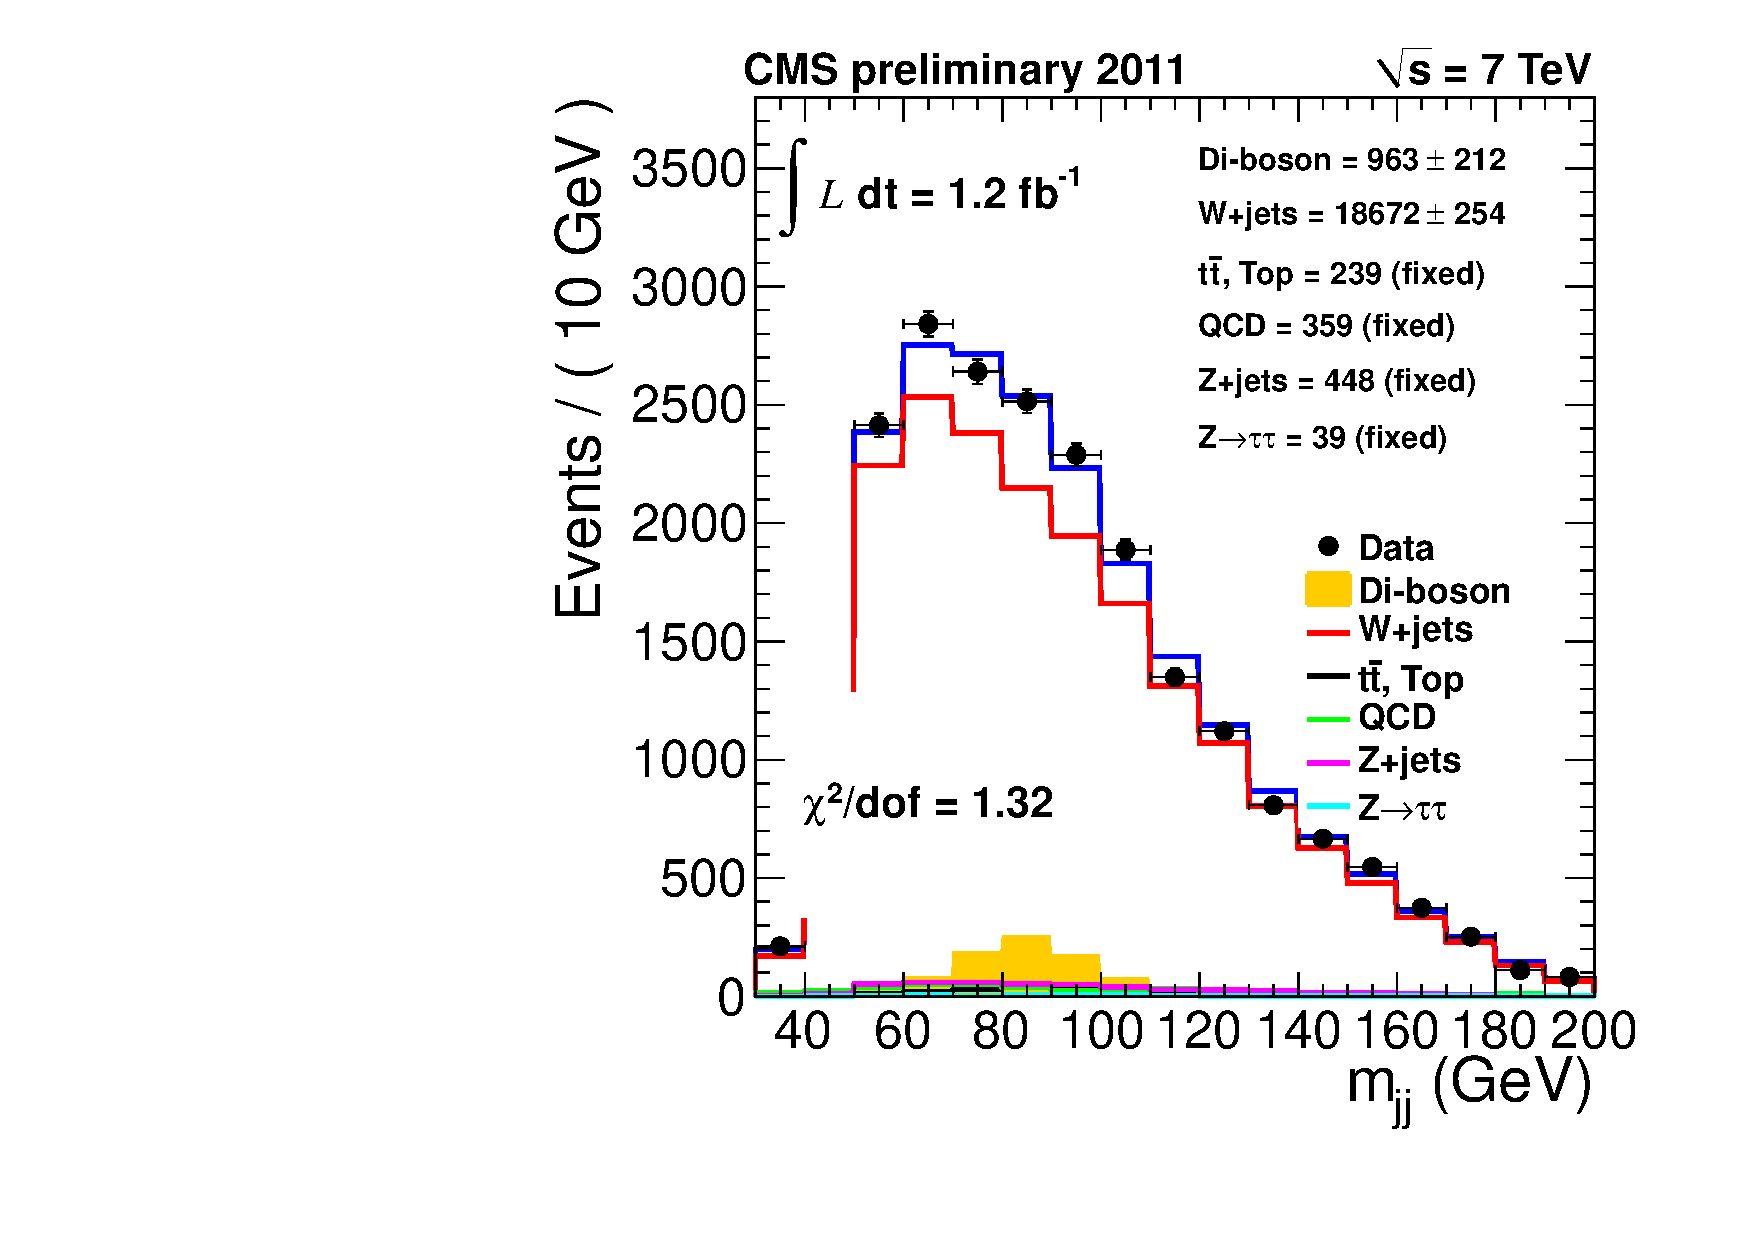
\includegraphics[width=0.31\textwidth]{figs/CDFtoWW_s4_mJJ-combined-fit.pdf} 
\unitlength=0.33\linewidth
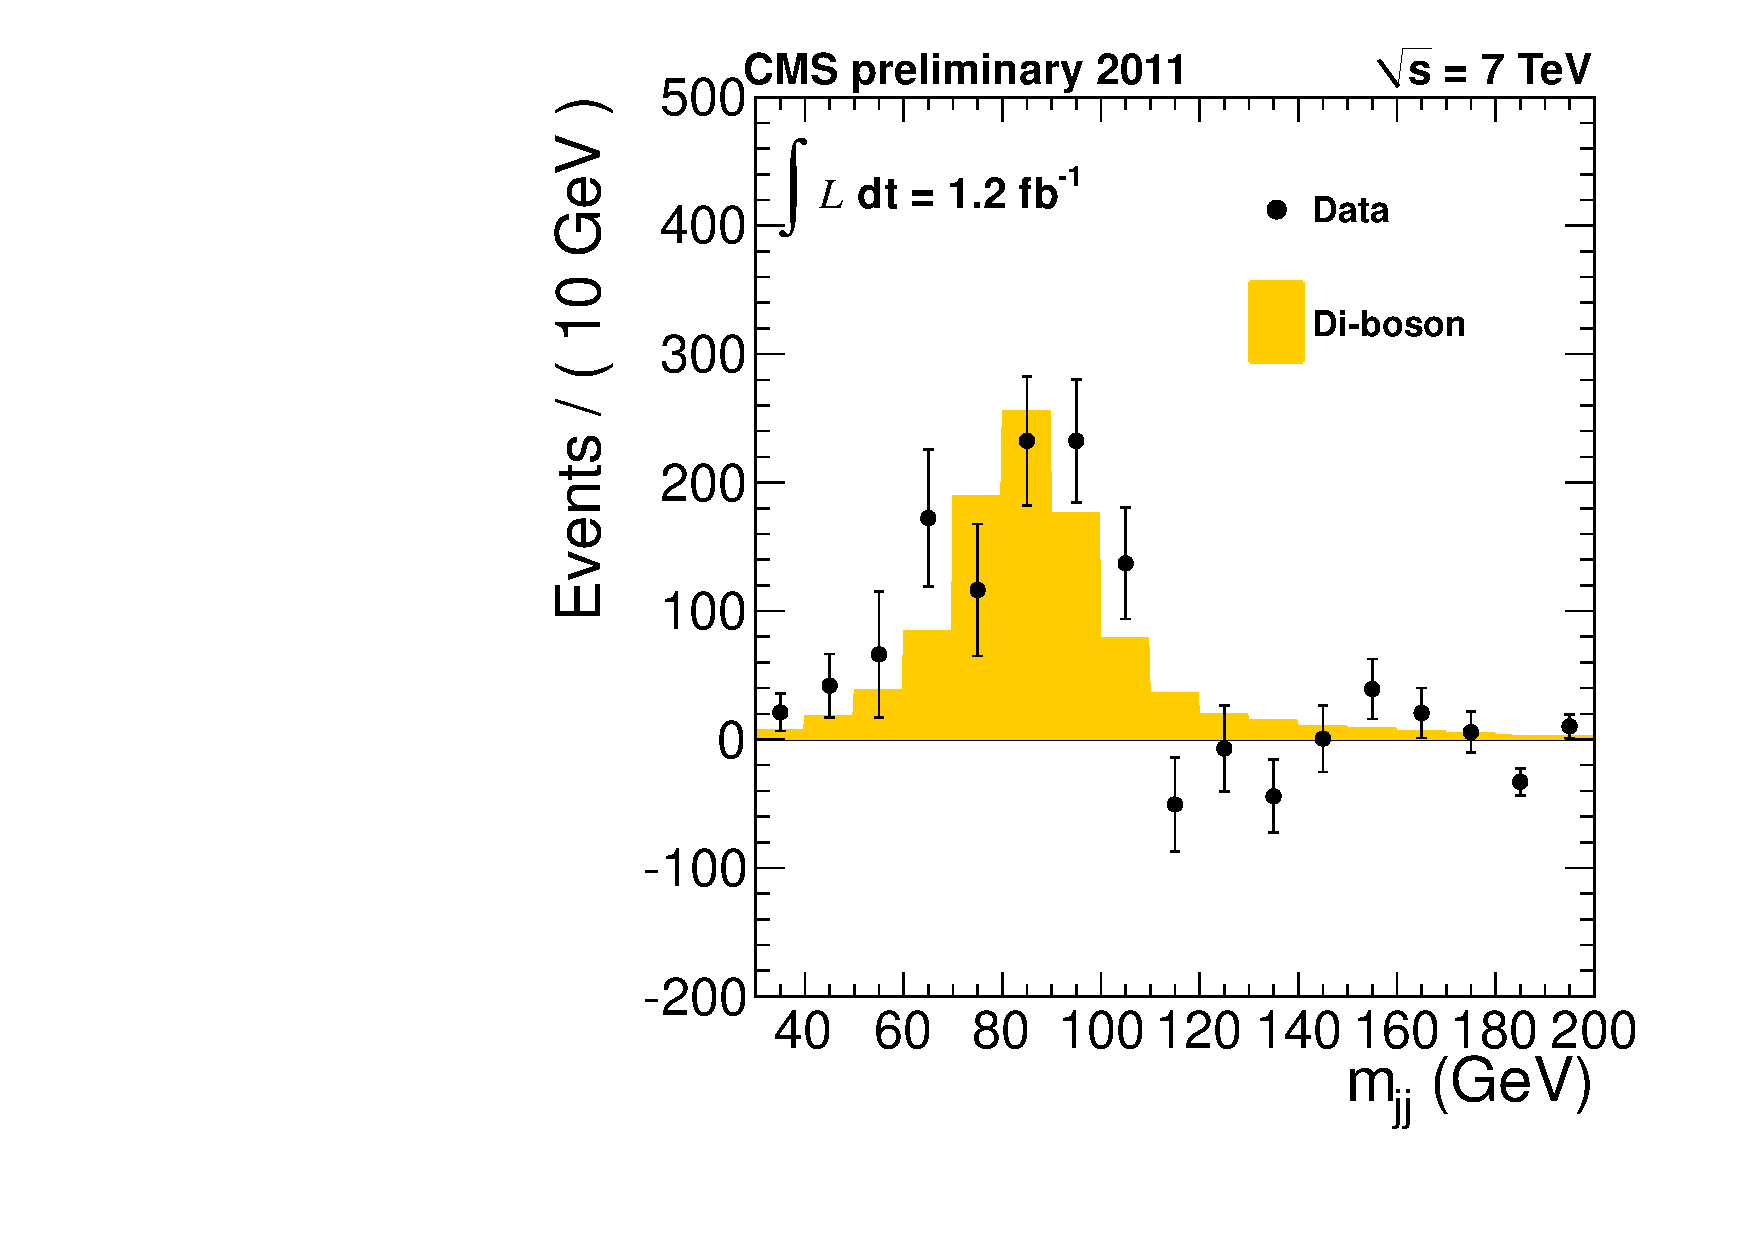
\includegraphics[width=0.31\textwidth]{figs/CDFtoWW_s4_mJJ-combined-fit-subtracted.pdf} 
\unitlength=0.33\linewidth
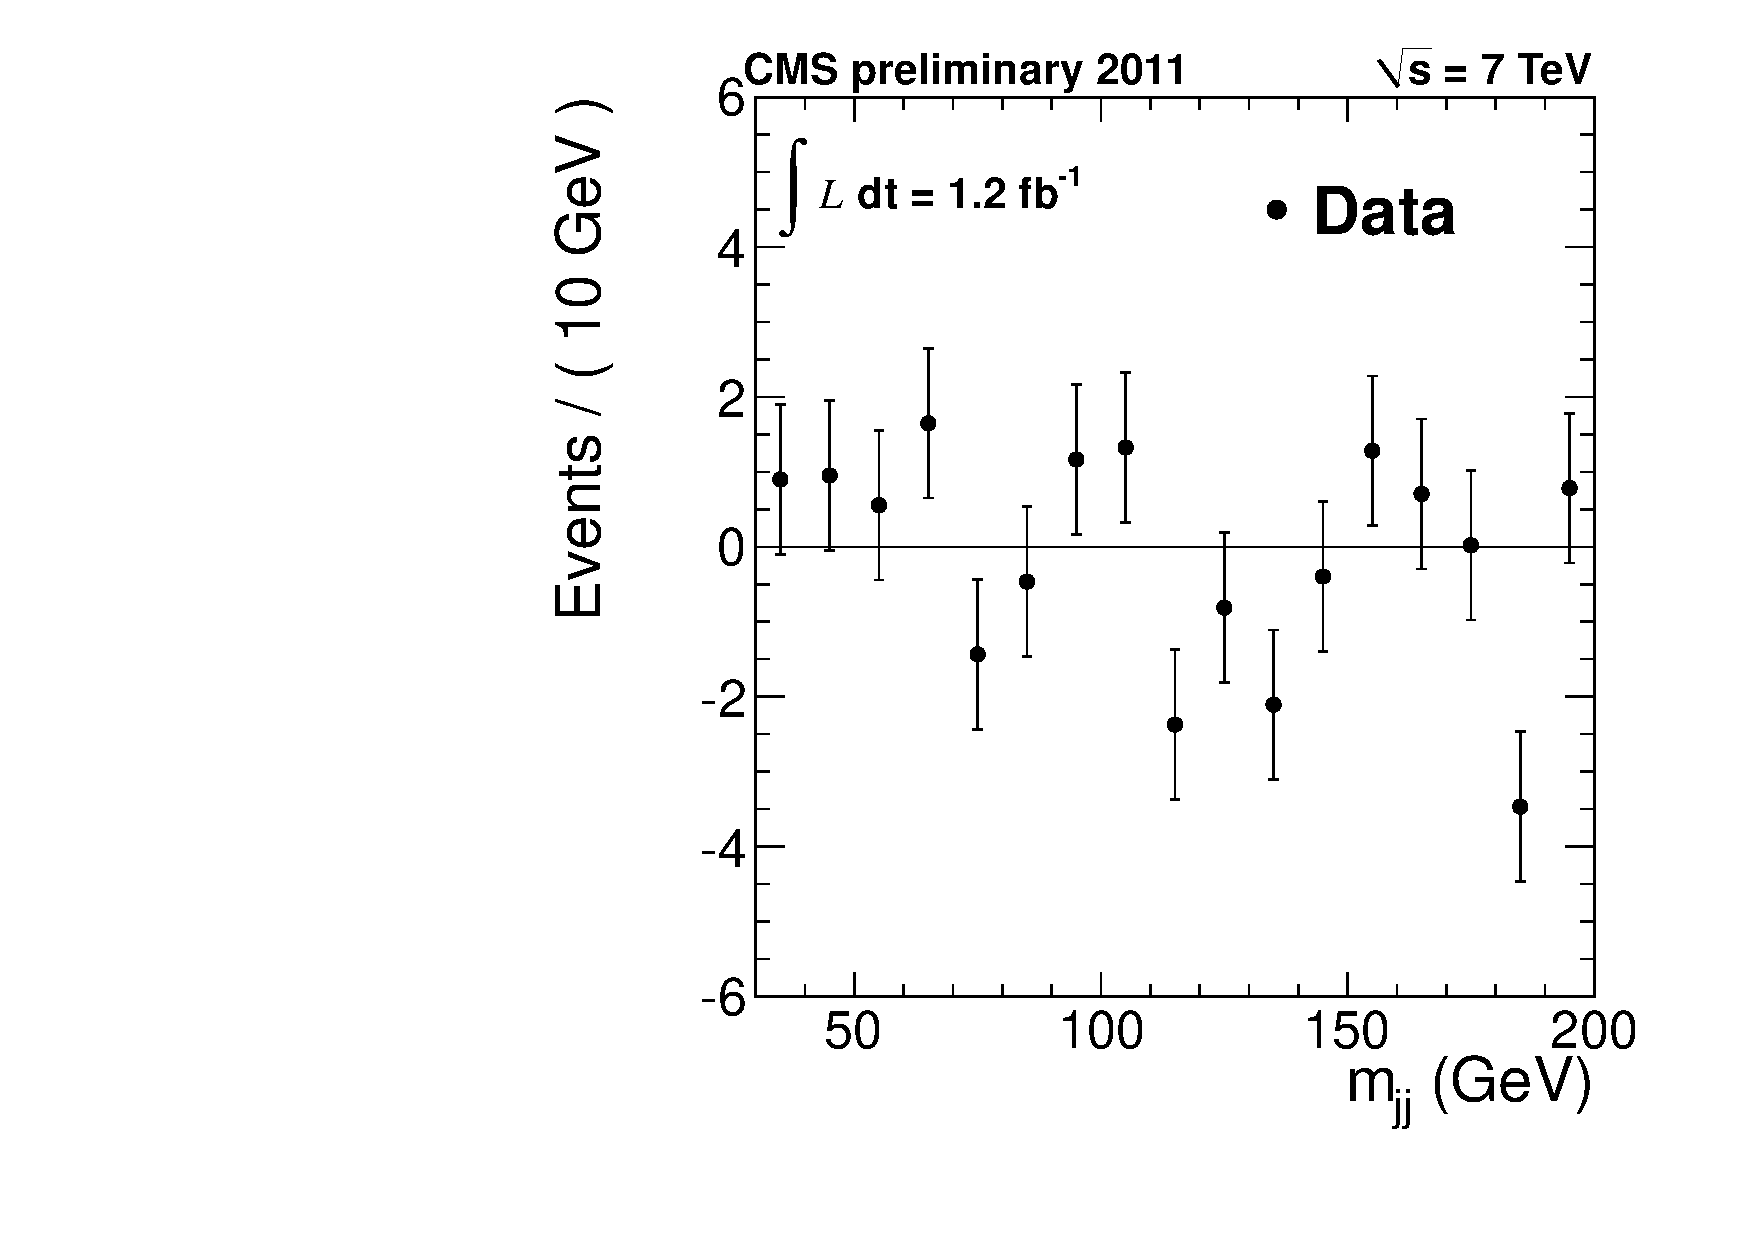
\includegraphics[width=0.31\textwidth]{figs/CDFtoWW_s4_mJJ-combined-fit-residual.pdf} \\
%%\put(-0.50,0.0){e)} \\
\caption{Fit results when making the transition from CDF-like to Diboson Analysis: a) CDF-like cuts, b) Kinematic Fit $\chi^2/NDF<10.0$, c) $-0.6<\cos (\textrm{JacksonAngle})<0.8$, d) $Jet2_{p_T}/m_{jj}>0.3$, e) Anti-$b$-tag (medium, highefficiency, Simple Secondary Vertex).} 
\label{fig:CDFtoWWcuts}}
\end{figure}
%%%%%%%
%%%%%%%%%%%%%%%%%%%%%%%%%%%%
